% DM d'optimisation (CentraleSupélec) -- décodage spéculatif
% Compilation : pdflatex rapport_dm.tex (deux passes pour les références croisées)
\documentclass[11pt,a4paper]{article}
\usepackage[utf8]{inputenc}
\usepackage[T1]{fontenc}
\usepackage{lmodern}
\usepackage[french]{babel}
\frenchsetup{SmallCapsFigTabCaptions=false,og=«,fg=»}
\usepackage[a4paper,margin=2.2cm]{geometry}
\usepackage{amsmath,amssymb,amsthm,mathtools}
\usepackage{graphicx}
\usepackage{booktabs,tabularx,array}
\usepackage{enumitem}
\usepackage{calc}
\usepackage[dvipsnames]{xcolor}
\usepackage{microtype}
\usepackage{caption}
\usepackage[colorlinks=true,linkcolor=MidnightBlue,citecolor=MidnightBlue,urlcolor=MidnightBlue]{hyperref}
\usepackage{xurl}

\captionsetup{font=small,labelfont=bf,format=hang,justification=justified}
\setlist{itemsep=2pt,topsep=3pt}
\setlength{\parskip}{3pt}
\graphicspath{{figures/}}

\newcommand{\R}{\mathbb{R}}
\newcommand{\TV}{\mathrm{TV}}
\newcommand{\Prob}{\mathbb{P}}
\newcommand{\Esp}{\mathbb{E}}
\newcommand{\sca}[2]{\langle #1,#2\rangle}
\newcommand{\nr}[1]{\|#1\|}
\newcommand{\clip}{\operatorname{clip}}
\newcommand{\vecop}{\operatorname{vec}}
\newcommand{\diag}{\operatorname{diag}}
\newcommand{\rg}{\operatorname{rg}}
\newcommand{\cB}{\mathcal{B}}
\newcommand{\cN}{\mathcal{N}}
\newcommand{\barre}[1]{\leavevmode\rlap{\rule[0.55ex]{\widthof{#1}}{0.5pt}}#1}
\newcommand{\tok}[1]{\texttt{#1}}

\theoremstyle{plain}
\newtheorem{proposition}{Proposition}
\newtheorem{lemme}{Lemme}
\theoremstyle{definition}
\newtheorem{exemple}{Exemple}
\newtheorem*{remarque}{Remarque}
\newtheorem*{suite}{Suite de l'exemple~\ref{ex:n3}}

\title{\textbf{Où relâcher la vérification ?}\\[2pt]
\large Allocation optimale d'un budget de déviation en décodage spéculatif}
\author{Prénom~Nom~1 \and Prénom~Nom~2\\[2pt]
\small DM d'optimisation, CentraleSupélec, dominante Mathématiques et Sciences des Données, 2026--2027}
\date{}

\begin{document}
\maketitle

\begin{abstract}
En décodage spéculatif, un petit modèle (le \emph{draft}) propose des tokens qu'un grand modèle (le \emph{target}) vérifie en une seule passe.
Nous formalisons deux problèmes d'optimisation issus de notre projet de recherche.
\textbf{(I)} Vérifier un token revient à résoudre un programme linéaire de transport. La dualité fournit un certificat explicite que l'acceptation maximale vaut $1-\TV(p,q)$, ce que confirme notre simplexe ; si l'on tolère une déviation $\varepsilon$ de la loi émise, elle passe à $\min(1,1-\TV+\varepsilon)$, et le prix dual d'une unité de déviation vaut~1.
\textbf{(II)} Répartir un budget de déviation entre les positions d'un bloc drafté est un problème \emph{non concave} sous contraintes linéaires. Nous écrivons les conditions KKT, résolvons le problème par gradient projeté et vérifions les conditions d'optimalité.
Résultat principal : comme un rejet termine le bloc, le budget doit aller en priorité aux \textbf{premières} positions, même lorsqu'elles sont plus sensibles ; dans un scénario typique, l'allocation optimale est 26\,\% plus rapide qu'un modèle qui ignore cette structure.
\end{abstract}

\begin{center}
\small
\begin{tabularx}{\linewidth}{@{}>{\raggedright}p{0.36\linewidth}X@{}}
\toprule
\textbf{Attendu du DM} & \textbf{Où} \\\midrule
Modélisation (variables, objectif, contraintes) & §\ref{sec:contexte}, §\ref{sec:modeleI}, §\ref{sec:modeleII}\\
Existence et unicité & §\ref{sec:existenceI} (PL), §\ref{sec:existenceII} (compacité, non-concavité, cas $\gamma=2$)\\
Théorèmes du cours, conditions d'optimalité & dualité en PL (§\ref{sec:dualite}), conditions KKT, Th.~2.5.17 (§\ref{sec:kkt}), inéquation d'Euler, Th.~2.5.1 (annexe~\ref{app:convergence})\\
Choix de l'algorithme et convergence & simplexe en deux phases (§\ref{sec:simplexe}), gradient projeté (§\ref{sec:algoII} et annexe~\ref{app:convergence})\\
Plusieurs minima locaux ? & §\ref{sec:algoII} : objectif non concave, multi-départs systématiques\\
Points d'originalité & \textbf{méthode du simplexe}, \textbf{mise en œuvre de la dualité} (certificat, prix duaux), objectif non concave\\
\bottomrule
\end{tabularx}
\end{center}

%=====================================================================
\section{Contexte et notations}\label{sec:contexte}
%=====================================================================
À chaque position, le target définit une loi $p$ sur le vocabulaire et le draft une loi $q$.
La règle de Leviathan et al.~\cite{leviathan} (proposée indépendamment par Chen et al.~\cite{chen}) accepte le token drafté $x\sim q$ avec probabilité $\min(1,p_x/q_x)$ ; en cas de rejet, elle ré-échantillonne dans $(p-q)_+$ normalisée, et la loi émise est alors exactement $p$.
Le draft propose un bloc de $\gamma$ tokens, que le target vérifie en \emph{une} passe ; le premier rejet termine le bloc.
La vitesse se mesure par le nombre moyen de tokens produits par passe du target.
Une vérification \emph{avec perte}~\cite{fuzzy} accepte plus souvent, au prix d'une déformation de la loi émise ; notre projet de recherche cherche \emph{où} cette déformation est sans danger pour la réponse finale.
On note $\TV(p,q)=\tfrac12\nr{p-q}_1$ et $\beta(p,q)=\sum_i\min(p_i,q_i)=1-\TV(p,q)$ (identité démontrée au §\ref{sec:existenceI}).

\paragraph{Exemple concret (Qwen2.5-0.5B propose, Qwen2.5-1.5B vérifie, GSM8K).}
Le draft propose 5 tokens ; le target les vérifie en une passe, garde les tokens jusqu'au premier désaccord, puis écrit le sien (vérification gloutonne).
Problème A : « Sofie marche deux fois plus que Brian\dots » ; problème B : « trois bâtons de colle, il en reste 1/6, 2/3 et 1/2\dots ».
Le token barré est celui du draft, le token en gras celui du target ; la colonne $\min(1,p_x/q_x)$ donne la probabilité avec laquelle la règle stochastique de~\cite{leviathan} aurait quand même accepté le token rejeté.

\begin{center}
\small
\begin{tabularx}{\linewidth}{@{}c>{\raggedright}p{0.32\linewidth}ccX@{}}
\toprule
Pb & Bloc proposé par le draft & Acceptés & $\min(1,p_x/q_x)$ & Lecture\\\midrule
A & \tok{To \barre{determine}} $\to$ \tok{\textbf{find}}\dots & 1/5 & 0,59 & synonyme : sans effet sur la réponse\\
A & \tok{out how many miles Brian} & 5/5 & -- & bloc entier accepté : 6 tokens pour une passe\\
B & \tok{we need to \barre{follow}} $\to$ \tok{\textbf{calculate}}\dots & 3/5 & 0,17 & synonyme : sans effet sur la réponse\\
A & \tok{10 miles every day} & 5/5 & -- & nombres recopiés de l'énoncé : acceptés\\
B & \tok{is \barre{not}} $\to$ \tok{\textbf{left}}\dots & 1/5 & 0,24 & \textbf{pivot} : « ce qui est utilisé » ou « ce qui reste »\\
A & \tok{the distance \barre{Brian}} $\to$ \tok{\textbf{Sof}}\dots & 2/5 & 0,43 & \textbf{pivot} : distance de Brian ou de Sofie\\
\bottomrule
\end{tabularx}
\end{center}

Sur ces deux solutions, le target produit en moyenne 4,76 et 4,59 tokens par passe, au lieu de 1 sans draft.
La plupart des rejets portent sur des \textbf{synonymes} sans effet sur la réponse : c'est là qu'une vérification avec perte gagnerait de la vitesse sans risque.
Quelques rejets portent sur des \textbf{pivots} qui orientent le raisonnement : c'est là qu'il ne faut pas relâcher.
Ce DM formalise ce compromis.

%=====================================================================
\section{Partie I : vérifier un token est un programme linéaire}
%=====================================================================
\subsection{Modèle : variables, objectif, contraintes}\label{sec:modeleI}
\paragraph{Variables.} Une règle de vérification (exacte ou non) est entièrement décrite par la loi jointe du couple (token proposé par le draft, token finalement émis) :
\[\pi\in\R_+^{n\times n},\qquad \pi_{xy}=\Prob(\text{le draft propose }x\text{ et l'on émet }y).\]
On accepte le token du draft exactement quand $y=x$ : la probabilité d'acceptation est la somme des cases \emph{diagonales} de $\pi$.

\paragraph{Contraintes.} (i) Le draft propose selon sa loi : la somme de la ligne $x$ vaut $q_x$. (ii) La règle est exacte si le token émis suit la loi du target : la somme de la colonne $y$ vaut $p_y$. (iii) $\pi\ge0$. D'où
\[(P_0)\qquad \max_{\pi\ge0}\ \sum_x\pi_{xx}\quad\text{s.c.}\quad \sum_y\pi_{xy}=q_x\ \ (x=1,\dots,n),\qquad \sum_x\pi_{xy}=p_y\ \ (y=1,\dots,n).\]

\paragraph{Forme standard du cours} ($\min c\cdot x$, $Ax=b$, $x\ge0$). On range les $n^2$ inconnues ligne par ligne : $\vecop(\pi)=(\pi_{11},\dots,\pi_{1n},\pi_{21},\dots,\pi_{nn})$.
\begin{itemize}
\item \textbf{Coût.} Maximiser $\sum_x\pi_{xx}$ revient à minimiser son opposé : $c=-\vecop(I_n)$ vaut $-1$ sur les $n$ composantes diagonales et $0$ ailleurs, de sorte que $c\cdot\pi=-\text{acceptation}$.
\item \textbf{Matrice $A\in\{0,1\}^{2n\times n^2}$ et second membre $b=(q,p)\in\R^{2n}$} : une colonne par variable $\pi_{xy}$, une ligne par contrainte. Pour $n=3$ :
\end{itemize}
\begin{center}\small
$\begin{array}{r|ccc|ccc|ccc|c}
 & \pi_{11} & \pi_{12} & \pi_{13} & \pi_{21} & \pi_{22} & \pi_{23} & \pi_{31} & \pi_{32} & \pi_{33} & b\\\hline
\text{ligne }x=1 & 1 & 1 & 1 & 0 & 0 & 0 & 0 & 0 & 0 & q_1\\
\text{ligne }x=2 & 0 & 0 & 0 & 1 & 1 & 1 & 0 & 0 & 0 & q_2\\
\text{ligne }x=3 & 0 & 0 & 0 & 0 & 0 & 0 & 1 & 1 & 1 & q_3\\\hline
\text{colonne }y=1 & 1 & 0 & 0 & 1 & 0 & 0 & 1 & 0 & 0 & p_1\\
\text{colonne }y=2 & 0 & 1 & 0 & 0 & 1 & 0 & 0 & 1 & 0 & p_2\\
\text{colonne }y=3 & 0 & 0 & 1 & 0 & 0 & 1 & 0 & 0 & 1 & p_3
\end{array}$
\end{center}

\paragraph{Trois propriétés de $A$.}
\begin{enumerate}
\item \textbf{Structure de flot.} Chaque colonne contient exactement deux 1 : $\pi_{xy}$ intervient dans la contrainte « ligne $x$ » et dans la contrainte « colonne $y$ ». En multipliant par $-1$ les $n$ lignes « colonne », chaque colonne contient un $+1$ et un $-1$ : c'est la matrice d'incidence d'un graphe orienté biparti (tokens proposés $\to$ tokens émis), totalement unimodulaire par le lemme de Poincaré (Lemme~4.3.5) ; changer le signe d'une ligne ne change que le signe des déterminants, donc $A$ est aussi TU. Comme $b=(q,p)$ n'est pas entier, cette propriété ne sert pas ici à l'intégrité : elle situe simplement $(P_0)$ parmi les problèmes de flot du cours.
\item \textbf{Rang.} $\rg(A)=2n-1$. La somme des $n$ lignes du haut et celle des $n$ lignes du bas valent toutes deux $(1,\dots,1)$ : une ligne est redondante, donc $\rg(A)\le2n-1$. Réciproquement, si l'on retire la contrainte « colonne 1 », les $2n-1$ colonnes associées à $\pi_{11}$, aux $\pi_{1y}$ ($y\ge2$) et aux $\pi_{x1}$ ($x\ge2$) engendrent tous les vecteurs de base de $\R^{2n-1}$ : $\rg(A)=2n-1$. Le cours suppose $A$ de rang égal à son nombre de lignes ; le code retire donc une ligne avant le simplexe.
\item \textbf{Compatibilité.} Le système n'a de solution que si $\sum_xq_x=\sum_yp_y$ (les deux valent la masse totale $\sum_{x,y}\pi_{xy}$), ce qui est vrai pour deux lois. Sur les données réelles, les sommes valent $1\pm10^{-6}$ (arrondis du softmax en float32) : on renormalise, faute de quoi le PL est réellement non admissible.
\end{enumerate}

\subsection{Existence, valeur et (non-)unicité}\label{sec:existenceI}
\paragraph{Existence.} L'ensemble admissible est \textbf{non vide} (le couplage indépendant $\pi_{xy}=q_xp_y$ vérifie $\sum_yq_xp_y=q_x$ et $\sum_xq_xp_y=p_y$) et \textbf{borné} ($0\le\pi_{xy}\le\sum_{y'}\pi_{xy'}=q_x\le1$). C'est donc un polyèdre compact ; l'objectif est linéaire, donc continu, et le maximum est atteint (Th.~2.2.1). La Prop.~4.2.6 du cours garantit de plus l'existence d'une \textbf{solution basique optimale} (un sommet du polyèdre). La figure~\ref{fig:lp} illustre la proposition ci-dessous : valeur du PL (a, voir le §\ref{sec:validation}) et deux solutions optimales distinctes (b-c).

\begin{figure}[htbp]
\centering
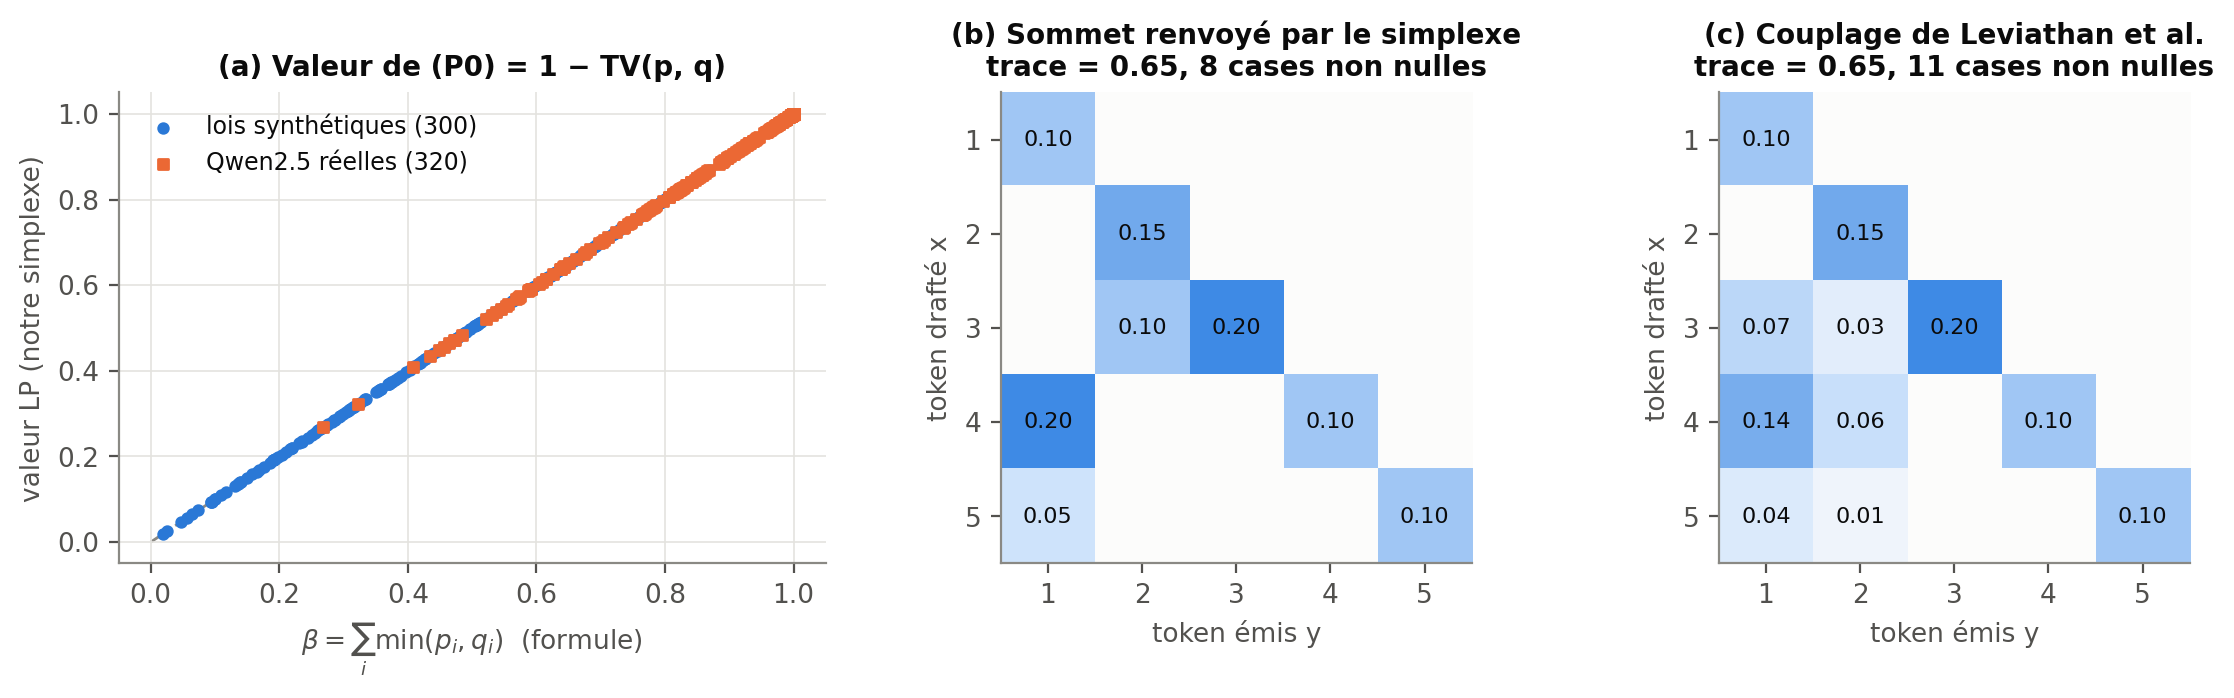
\includegraphics[width=\linewidth]{fig1_lp_exact.png}
\caption{(a) La valeur de $(P_0)$ calculée par notre simplexe coïncide avec $\beta=\sum\min(p,q)$. (b-c) Deux couplages optimaux pour $p=(0{,}35;0{,}25;0{,}2;0{,}1;0{,}1)$ et $q=(0{,}1;0{,}15;0{,}3;0{,}3;0{,}15)$ : même diagonale, partie hors diagonale différente.}
\label{fig:lp}
\end{figure}

\begin{proposition}[valeur de $(P_0)$]\label{prop:valeur}
La valeur optimale de $(P_0)$ vaut $\beta(p,q)=\sum_x\min(p_x,q_x)=1-\TV(p,q)$.
Les solutions optimales sont exactement les $\pi\ge0$ telles que $\pi_{xx}=\min(p_x,q_x)$ pour tout $x$ et dont la partie hors diagonale a pour marges $(q-p)_+$ (lignes) et $(p-q)_+$ (colonnes).
La solution est unique si et seulement si l'un de ces deux vecteurs a au plus une composante non nulle.
\end{proposition}

\paragraph{Deux identités utilisées partout.} Pour deux réels $a,b$ : $\min(a,b)+(a-b)_+=a$ (cas $a\le b$ et $a>b$). Pour deux lois $p,q$ :
\[\sum_x(p_x-q_x)_+=\sum_x(q_x-p_x)_+=\TV(p,q),\]
car la différence de ces deux sommes vaut $\sum_x(p_x-q_x)=0$ et leur somme $\sum_x|p_x-q_x|=2\,\TV$. On en déduit $\beta=\sum_x\big(p_x-(p_x-q_x)_+\big)=1-\TV$.

\begin{proof}
\emph{Étape 1 : majoration.} Pour tout $\pi$ admissible, une case diagonale est inférieure à la somme de sa ligne et à celle de sa colonne (les autres cases sont $\ge0$) : $\pi_{xx}\le q_x$ et $\pi_{xx}\le p_x$, donc $\sum_x\pi_{xx}\le\beta$.

\emph{Étape 2 : la borne est atteinte par le couplage de Leviathan.} Si $\TV=0$, alors $p=q$ et $\diag(p)$ convient. Sinon, la règle de~\cite{leviathan} accepte $x$ avec probabilité $\min(1,p_x/q_x)$, et sinon tire $y$ selon $(p-q)_+/\TV$ ; elle induit le couplage
\[\pi^L=\underbrace{\diag\big(\min(p,q)\big)}_{\text{proposer }x\text{ et l'accepter}}+\underbrace{\frac{(q-p)_+\,(p-q)_+^{\top}}{\TV}}_{\text{proposer }x,\text{ rejeter, émettre }y}.\]
\begin{itemize}
\item Diagonale : $\Prob(\text{proposer }x\text{ et accepter})=q_x\min(1,p_x/q_x)=\min(p_x,q_x)$.
\item Hors diagonale : $\Prob(\text{proposer }x\text{ et rejeter})=q_x-\min(p_x,q_x)=(q_x-p_x)_+$, puis $y$ est tiré avec probabilité $(p_y-q_y)_+/\TV$.
\item Lignes : $\sum_y\pi^L_{xy}=\min(p_x,q_x)+(q_x-p_x)_+\,\frac{\sum_y(p_y-q_y)_+}{\TV}=\min(p_x,q_x)+(q_x-p_x)_+=q_x$.
\item Colonnes : $\sum_x\pi^L_{xy}=\min(p_y,q_y)+\frac{\sum_x(q_x-p_x)_+}{\TV}\,(p_y-q_y)_+=p_y$.
\item Trace : le terme de rang 1 est nul sur la diagonale, car $(q_x-p_x)_+(p_x-q_x)_+=0$. Donc $\sum_x\pi^L_{xx}=\beta$.
\end{itemize}
$\pi^L$ est admissible et atteint la borne de l'étape 1 : il est optimal, et la valeur de $(P_0)$ est $\beta$.

\emph{Étape 3 : forme de toutes les solutions.} Si $\pi$ est optimal, $\sum_x\pi_{xx}=\beta$ alors que $\pi_{xx}\le\min(p_x,q_x)$ pour tout $x$ : toutes ces inégalités sont des égalités. Il reste sur la ligne $x$ la masse $(q_x-p_x)_+$ et sur la colonne $y$ la masse $(p_y-q_y)_+$, à répartir hors diagonale (figure~\ref{fig:structure}). Une case $\pi_{xy}>0$ hors diagonale exige $q_x>p_x$ et $p_y>q_y$ ; ces deux ensembles étant disjoints, on a bien $x\ne y$. Réciproquement, tout $\pi\ge0$ de cette forme a les bonnes marges et la trace $\beta$.

\emph{Étape 4 : (non-)unicité.} Supposons que $\{q>p\}$ et $\{p>q\}$ contiennent chacun au moins deux tokens. Il existe alors $x\ne x'$ dans $\{q>p\}$ et $y\ne y'$ dans $\{p>q\}$ avec $\pi_{xy}>0$ et $\pi_{x'y'}>0$. En effet, chaque colonne $y\in\{p>q\}$ reçoit une masse $>0$, donc il existe $\pi_{x_1y_1}>0$ et $\pi_{x_2y_2}>0$ avec $y_1\ne y_2$ ; si $x_1\ne x_2$, c'est terminé ; sinon on prend une autre ligne $x'\in\{q>p\}$, qui a une case $\pi_{x'y''}>0$ avec $y''$ différent de $y_1$ ou de $y_2$, et l'on associe ces deux cases.
On remplace alors $\pi_{xy},\pi_{x'y'}$ par $\pi_{xy}-\delta,\pi_{x'y'}-\delta$ et $\pi_{xy'},\pi_{x'y}$ par $\pi_{xy'}+\delta,\pi_{x'y}+\delta$, avec $0<\delta\le\min(\pi_{xy},\pi_{x'y'})$ : chaque ligne et chaque colonne gagne et perd $\delta$, la diagonale est inchangée (les quatre cases sont hors diagonale, car $\{q>p\}$ et $\{p>q\}$ sont disjoints), et l'on obtient une autre solution optimale (figure~\ref{fig:cycle}).
Si l'un des deux supports a au plus un élément, la partie hors diagonale est forcée (toute la masse va vers, ou vient de, ce seul token, ou il n'y a rien à placer) : la solution est unique.
\end{proof}

\begin{figure}[htbp]
\centering
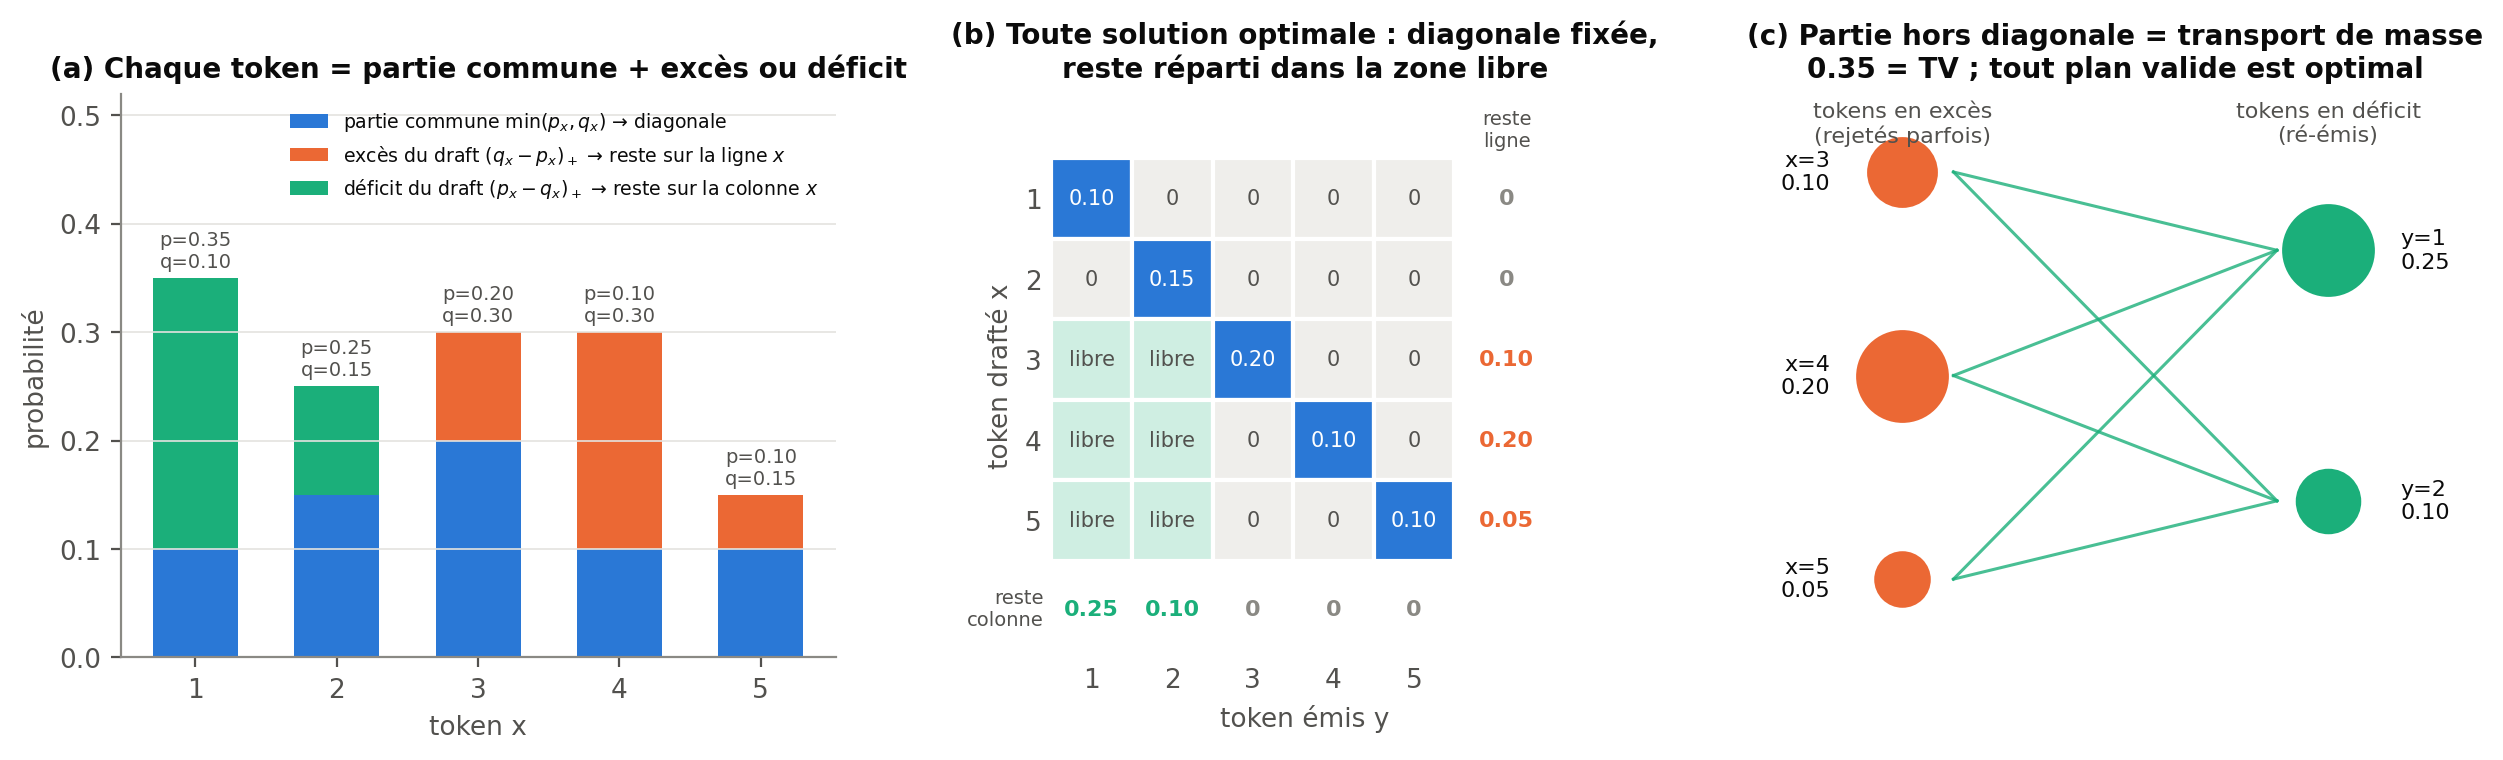
\includegraphics[width=\linewidth]{fig1b_structure.png}
\caption{\emph{Étape 3 de la preuve}, sur l'exemple de la figure~\ref{fig:lp} : $p=(0{,}35;0{,}25;0{,}2;0{,}1;0{,}1)$, $q=(0{,}1;0{,}15;0{,}3;0{,}3;0{,}15)$.
(a) Chaque token se décompose en une partie commune $\min(p_x,q_x)$ (bleu), qui va sur la diagonale de $\pi$, plus soit un excès du draft $(q_x-p_x)_+$ (orange), soit un déficit $(p_x-q_x)_+$ (vert).
(b) Structure imposée à toute solution optimale : diagonale fixée à $\min(p,q)$ ; il reste $(q-p)_+$ à placer sur chaque ligne et $(p-q)_+$ sur chaque colonne. Une case hors diagonale ne peut être non nulle que si sa ligne a un reste et sa colonne un besoin (cases « libres » : lignes 3 à 5, colonnes 1 et 2).
(c) Remplir la zone libre revient à transporter la masse $\TV=0{,}35$ des tokens en excès vers les tokens en déficit ; tout plan qui respecte ces masses donne la même acceptation $\beta=0{,}65$.}
\label{fig:structure}
\end{figure}

\begin{figure}[htbp]
\centering
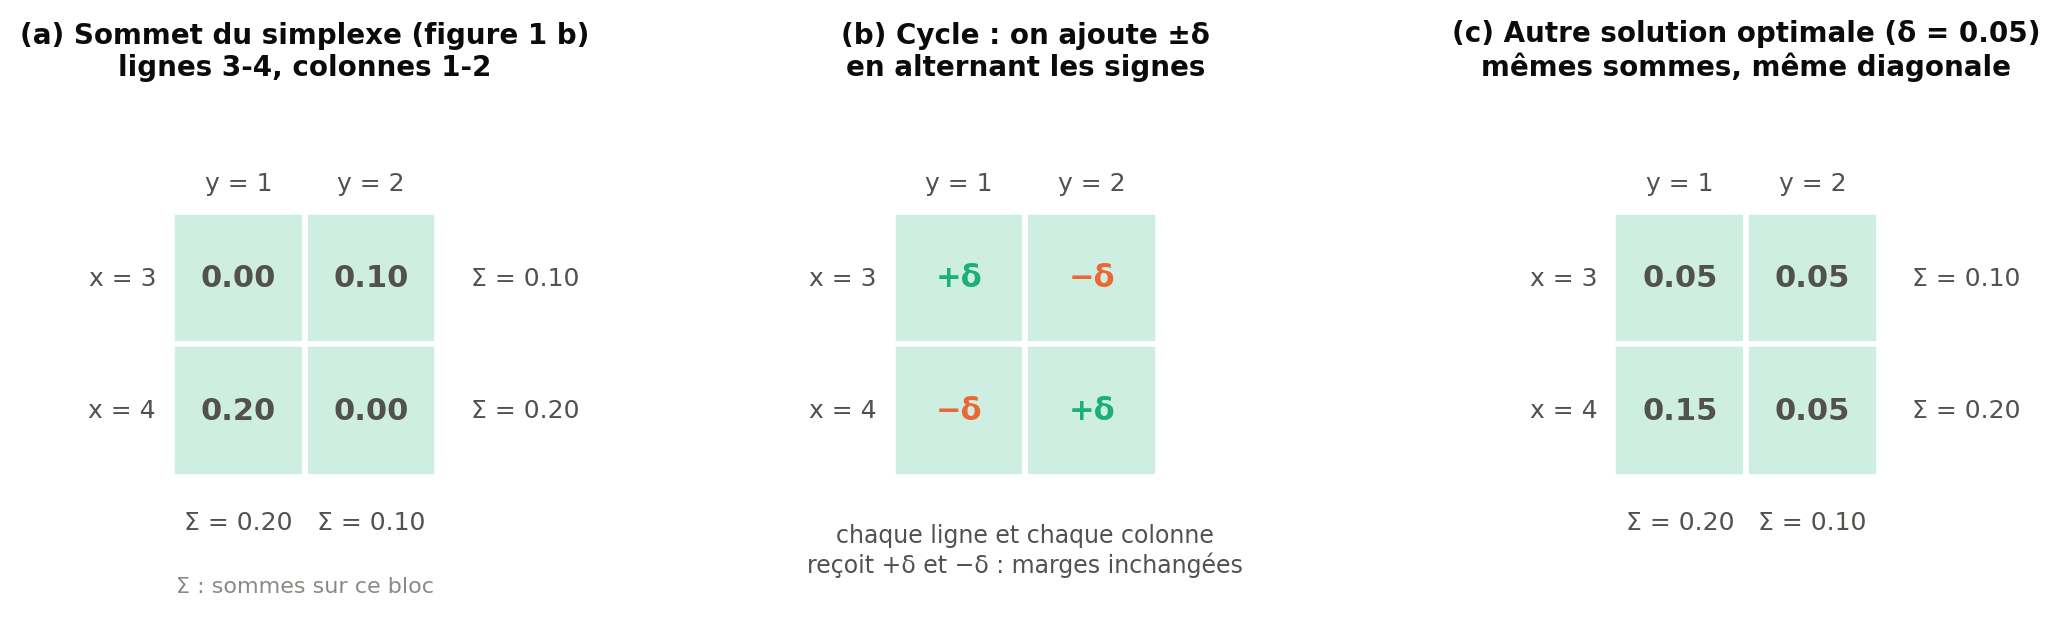
\includegraphics[width=0.92\linewidth]{fig1c_cycle.png}
\caption{\emph{Étape 4 de la preuve.} (a) Bloc lignes 3--4 $\times$ colonnes 1--2 du sommet renvoyé par le simplexe. (b) On ajoute $+\delta$ et $-\delta$ en alternant les signes : chaque ligne et chaque colonne du bloc gagne et perd $\delta$. (c) Avec $\delta=0{,}05$, on obtient une autre solution admissible avec la même diagonale, donc la même acceptation $\beta=0{,}65$ : il y a une infinité de solutions optimales. Ce cycle n'existe pas si un seul token est en excès ou un seul en déficit (exemple~\ref{ex:n3}).}
\label{fig:cycle}
\end{figure}

\begin{exemple}[$n=3$]\label{ex:n3}
Target $p=(0{,}5;0{,}3;0{,}2)$, draft $q=(0{,}2;0{,}3;0{,}5)$.
On a $\min(p,q)=(0{,}2;0{,}3;0{,}2)$, donc $\beta=0{,}7$ et $\TV=0{,}3$ ; $(q-p)_+=(0;0;0{,}3)$ (le draft sur-propose le token 3) et $(p-q)_+=(0{,}3;0;0)$ (il sous-propose le token 1).
\[\pi^L=\begin{pmatrix}0{,}2&0&0\\0&0{,}3&0\\\mathbf{0{,}3}&0&0{,}2\end{pmatrix}:\]
la case en gras se lit « le draft propose 3 alors que le target préfère 1 : on rejette et on émet 1 ». Lignes $(0{,}2;0{,}3;0{,}5)=q$, colonnes $(0{,}5;0{,}3;0{,}2)=p$, trace $0{,}7=\beta$. Chaque support est un singleton : la solution optimale est unique.
\end{exemple}

\subsection{Dualité : un certificat d'optimalité explicite}\label{sec:dualite}
\paragraph{Écriture du dual.} Le dual de $\min\{c\cdot x:Ax=b,\ x\ge0\}$ est $\max\{b\cdot\mu:A^\top\mu\le c\}$ (Th.~4.2.13). On note $\mu=(\varphi,\psi)\in\R^n\times\R^n$, où $\varphi_x$ est le multiplicateur de la contrainte « ligne $x$ » et $\psi_y$ celui de « colonne $y$ ». La colonne de $A$ associée à $\pi_{xy}$ contient un 1 sur la ligne $x$ et un 1 sur la ligne $n+y$, donc $(A^\top\mu)_{xy}=\varphi_x+\psi_y$ ; de plus $c_{xy}=-\delta_{xy}$ et $b\cdot\mu=q\cdot\varphi+p\cdot\psi$. D'où
\[(D_0)\qquad \max_{\varphi,\psi}\ q\cdot\varphi+p\cdot\psi\quad\text{s.c.}\quad \varphi_x+\psi_y\le-\delta_{xy}\quad\forall x,y.\]

\paragraph{Dualité faible, en une ligne.} Pour $\pi$ admissible et $\mu$ dual admissible, $c-A^\top\mu\ge0$ et $\pi\ge0$, donc
\[c\cdot\pi\ \ge\ (A^\top\mu)\cdot\pi=\mu\cdot(A\pi)=\mu\cdot b,\qquad\text{soit}\qquad -\sum_x\pi_{xx}\ \ge\ q\cdot\varphi+p\cdot\psi.\]
Si l'on exhibe $\pi$ et $\mu$ pour lesquels il y a égalité, les deux sont optimaux.

\paragraph{Le certificat.} Posons $S=\{x:q_x\le p_x\}$ (tokens que le draft ne sur-propose pas) et
\[\varphi_x=\begin{cases}-1&x\in S\\0&x\notin S\end{cases}\qquad \psi_y=\begin{cases}0&y\in S\\-1&y\notin S.\end{cases}\]
\begin{itemize}
\item Admissibilité sur la diagonale : exactement l'un des deux vaut $-1$, donc $\varphi_x+\psi_x=-1$.
\item Admissibilité hors diagonale : $\varphi_x+\psi_y\in\{0,-1,-2\}$, donc $\le0=c_{xy}$.
\item Valeur : $q\cdot\varphi+p\cdot\psi=-\sum_{x\in S}q_x-\sum_{y\notin S}p_y=-\sum_x\min(p_x,q_x)=-\beta$.
\end{itemize}
La valeur duale $-\beta$ égale la valeur primale $c\cdot\pi^L$ : par dualité faible, $\pi^L$ et $(\varphi,\psi)$ sont optimaux. On retrouve la proposition~\ref{prop:valeur} sans l'étape 1.

\paragraph{Écarts complémentaires.} À l'optimum, $\pi_{xy}>0\Rightarrow\varphi_x+\psi_y=c_{xy}$. Sur $\pi^L$ : une case hors diagonale non nulle a $q_x>p_x$ ($\varphi_x=0$) et $p_y>q_y$ ($\psi_y=0$), donc $\varphi_x+\psi_y=0=c_{xy}$ ; sur la diagonale, $\varphi_x+\psi_x=-1=c_{xx}$. \emph{Lecture :} $\varphi_x=-1$ marque les tokens que le draft propose « trop peu » ($q_x\le p_x$) : ils sont toujours acceptés.

\begin{suite}
$S=\{1,2\}$, donc $\varphi=(-1,-1,0)$ et $\psi=(0,0,-1)$ ; valeur duale $-(0{,}2+0{,}3)-0{,}2=-0{,}7=-\beta$.
\end{suite}

\subsection{Algorithme : simplexe révisé en deux phases}\label{sec:simplexe}
Le simplexe est programmé comme dans le cours (\texttt{specdm/simplex.py}). À chaque itération, avec l'ensemble de base $\cB$ (matrice $A_\cB$) et l'ensemble hors base $\cN$ :
\begin{enumerate}
\item solution de base $x_\cB=A_\cB^{-1}b$ et multiplicateurs $\mu=A_\cB^{-\top}c_\cB$ ;
\item coûts réduits $\tilde c_\cN=c_\cN-A_\cN^\top\mu$ ; si $\tilde c_\cN\ge0$, la base est optimale (Prop.~4.2.8) ;
\item sinon, la variable entrante $j$ a le coût réduit le plus négatif (règle de Dantzig) ; direction $d=A_\cB^{-1}A_j$, et le long de $x_\cB(\theta)=x_\cB-\theta d$ le coût baisse de $|\tilde c_j|\theta$ ;
\item test du ratio : $\theta^*=\min\{x_{\cB,i}/d_i:d_i>0\}$ ; si aucun $d_i>0$, le problème n'est pas borné, sinon la variable qui s'annule sort de la base.
\end{enumerate}
\textbf{Phase 1.} On résout $\min\mathbf1\cdot y$ sous $\tilde Ax+y=\tilde b$, $\tilde b=|b|$ (lignes de signe changé si besoin), en partant du sommet $(x,y)=(0,\tilde b)$ ; valeur nulle si et seulement si le problème est admissible, et la base finale, purgée des variables artificielles, démarre la phase 2.
\textbf{Dégénérescence.} Une base compte $2n-1$ variables, dont plusieurs sont souvent nulles ($\theta^*=0$ : pivot sans progrès). Pour exclure tout cyclage, on passe à la règle de Bland (plus petit indice) après $2m$ pivots dégénérés consécutifs ($m=2n-1$ est le nombre de contraintes).
Les multiplicateurs $\mu$ de la base finale forment la solution duale : c'est ainsi que l'on obtient les prix du §\ref{sec:perte}.

\subsection{Validation numérique}\label{sec:validation}
Nous vérifions trois choses distinctes : (i) l'implémentation du simplexe trouve le vrai optimum et le vrai dual ; (ii) la valeur du PL coïncide avec la formule $\beta$ ; (iii) le tout fonctionne sur de vraies lois de LLM.

\paragraph{Données synthétiques.} Pour chaque $n=3,\dots,12$, on tire 30 paires $(p,q)$ (300 au total), chaque loi suivant une loi de Dirichlet $\mathrm{Dir}(c,\dots,c)$ avec $c\in\{0{,}3;1;3\}$ : $c=0{,}3$ donne des lois très piquées (un LLM sûr de son prochain token), $c=3$ des lois presque uniformes. On couvre ainsi des paires très proches ($\beta\approx1$) comme très éloignées ($\beta\approx0$). Pour chaque paire, on compare la valeur de $(P_0)$ par \textbf{notre simplexe}, par \textbf{HiGHS} (solveur de référence de SciPy, développé indépendamment) et la \textbf{formule} $\beta$.

\begin{center}
\small
\begin{tabularx}{\linewidth}{@{}lcX@{}}
\toprule
Comparaison & Écart maximal & Lecture\\\midrule
notre simplexe / formule $\beta$ & $4{,}4\times10^{-16}$ & précision machine (en double précision, deux nombres proches de 1 ne se distinguent pas à moins de $2{,}2\times10^{-16}$ près)\\
HiGHS / formule $\beta$ & $4{,}4\times10^{-16}$ & idem\\
notre simplexe / formule, paires réelles & $3{,}5\times10^{-11}$ & voir ci-dessous\\
\bottomrule
\end{tabularx}
\end{center}

\paragraph{Vérification du dual.} Les tests unitaires (\texttt{tests/test\_specdm.py}) contrôlent, sur des PL aléatoires, l'\textbf{admissibilité duale} $A^\top\mu\le c$ et la \textbf{dualité forte} $b\cdot\mu=c\cdot x$ (à $10^{-8}$ près), comparent valeur et statut à HiGHS, et vérifient la détection des problèmes non admissibles et non bornés. Pour $(P_0)$, ils vérifient que le certificat $(\varphi,\psi)$ du §\ref{sec:dualite} est admissible et de valeur $-\beta$, que $\pi^L$ a les bonnes marges et que les écarts complémentaires sont satisfaits.

\paragraph{Coût du simplexe.} Nombre moyen d'itérations (phases 1 et 2) :
\begin{center}
\small
\begin{tabular}{@{}l*{10}{r}@{}}
\toprule
$n$ & 3 & 4 & 5 & 6 & 7 & 8 & 9 & 10 & 11 & 12\\
itérations & 10 & 16 & 21 & 31 & 38 & 47 & 58 & 75 & 87 & 105\\
\bottomrule
\end{tabular}
\end{center}
Le PL a $n^2$ variables et $2n-1$ contraintes indépendantes ; un ajustement en loi de puissance donne un exposant d'environ 1,7. Pour un vrai vocabulaire ($n\approx150\,000$), $(P_0)$ aurait plus de $2\times10^{10}$ variables : le simplexe sert ici à \emph{vérifier} la formule fermée $\beta$, que l'on calcule ensuite directement.

\paragraph{Données réelles.} On prend 320 positions tirées au hasard dans les solutions GSM8K (20 par problème) avec les lois $(p_t,q_t)$ des deux modèles Qwen2.5. Le vocabulaire étant trop grand pour le PL, on réduit chaque paire aux 6 tokens les plus probables de chaque modèle plus une case « autres » qui regroupe la masse restante (supports de 7 à 12 tokens). Deux précautions :
\begin{itemize}
\item \textbf{Renormalisation.} En float32, les sommes valent $1\pm10^{-6}$ ; or $(P_0)$ exige $\sum p=\sum q$ exactement : sans renormalisation, le PL est non admissible, et notre simplexe le détecte en phase 1.
\item \textbf{Écart de $3{,}5\times10^{-11}$.} Les lois réelles contiennent des masses minuscules (jusqu'à $10^{-12}$), plus petites que la tolérance $10^{-10}$ utilisée pour décider qu'un coût réduit est négatif : le simplexe s'arrête dès que le gain restant est inférieur à $10^{-10}$. L'écart reste négligeable devant toute quantité d'intérêt.
\end{itemize}

\paragraph{Portée de cette validation.} Elle ne remplace pas la preuve de la proposition~\ref{prop:valeur}, qui vaut pour toutes les lois ; elle détecte les erreurs d'implémentation, de formulation ou de données. Elle a d'ailleurs révélé deux points : les lois réelles non renormalisées rendaient le PL non admissible, et un test qui attendait un prix dual égal à 1 en $\varepsilon=0$ a échoué (le simplexe renvoyait 2) ; ce n'était pas une erreur mais un coin de la fonction valeur, où tout prix $\ge1$ est valide (§\ref{sec:perte}).

\paragraph{Non-unicité, observée.} Le simplexe renvoie un \textbf{sommet} (8 cases non nulles, au plus $2n-1=9$), tandis que $\pi^L$ est un autre optimum qui n'est pas un sommet (11 cases) ; les deux acceptent avec probabilité $0{,}65$ (figure~\ref{fig:lp}).

\subsection{Vérification avec perte et prix dual du budget}\label{sec:perte}
\paragraph{Modèle.} On autorise la loi émise $r$ à s'écarter de $p$ d'au plus $\varepsilon$ en variation totale : la seconde marge de $\pi$ devient une variable $r$ ($r_y=\sum_x\pi_{xy}\ge0$ et $\sum_yr_y=\sum_xq_x=1$ : $r$ est automatiquement une loi), avec $\TV(r,p)\le\varepsilon$. La valeur absolue n'étant pas linéaire, on introduit $t_y\ge0$ avec $t_y\ge r_y-p_y$ et $t_y\ge p_y-r_y$, c'est-à-dire $t_y\ge|r_y-p_y|$. Alors $\sum_yt_y\le2\varepsilon$ implique $\TV(r,p)\le\varepsilon$ ; réciproquement, si $\TV(r,p)\le\varepsilon$, le choix $t_y=|r_y-p_y|$ est admissible. Les deux formulations ont donc les mêmes $(\pi,r)$ admissibles :
\[(P_\varepsilon)\qquad \max_{\pi,r,t\ge0}\ \sum_x\pi_{xx}\quad\text{s.c.}\quad
\begin{aligned}&\textstyle\sum_y\pi_{xy}=q_x,\qquad \sum_x\pi_{xy}=r_y,\\
&t_y\ge r_y-p_y,\quad t_y\ge p_y-r_y,\qquad \textstyle\sum_yt_y\le2\varepsilon.\end{aligned}\]
En forme standard, chaque inégalité reçoit une variable d'écart positive ; la dernière ligne a pour second membre $2\varepsilon$.

\begin{proposition}[frontière avec perte]\label{prop:perte}
La valeur de $(P_\varepsilon)$ vaut $\alpha^*(\varepsilon)=\min(1,\beta+\varepsilon)$. Elle est atteinte par $r_\varepsilon=p+\theta(q-p)$ avec $\theta=\min(1,\varepsilon/\TV(p,q))$ (et $\theta=1$ si $\TV=0$).
\end{proposition}

\begin{proof}
\emph{Majoration.} Pour $(\pi,r,t)$ admissible, $\pi$ est un couplage des lois $q$ et $r$ : la proposition~\ref{prop:valeur} appliquée à $(q,r)$ donne $\sum_x\pi_{xx}\le1-\TV(q,r)$. L'inégalité triangulaire $\TV(q,p)\le\TV(q,r)+\TV(r,p)$ donne alors
\[\sum_x\pi_{xx}\ \le\ 1-\TV(q,p)+\TV(r,p)\ \le\ \beta+\varepsilon,\]
et bien sûr $\sum_x\pi_{xx}\le\sum_{x,y}\pi_{xy}=1$.

\emph{Borne atteinte.} $r_\varepsilon$ est un mélange de $p$ et $q$, donc une loi ; $r_\varepsilon-p=\theta(q-p)$ donne $\TV(r_\varepsilon,p)=\theta\,\TV\le\varepsilon$, et $q-r_\varepsilon=(1-\theta)(q-p)$ donne $\TV(q,r_\varepsilon)=(1-\theta)\TV$. Le couplage de Leviathan entre $q$ et $r_\varepsilon$ accepte avec probabilité
\[1-(1-\theta)\TV=\beta+\theta\,\TV=\begin{cases}\beta+\varepsilon&\text{si }\varepsilon\le\TV\ (\theta=\varepsilon/\TV),\\1&\text{si }\varepsilon\ge\TV\ (\theta=1,\ r_\varepsilon=q).\end{cases}\qedhere\]
\end{proof}

\begin{suite}[$\varepsilon=0{,}1$]
$\theta=1/3$, $r_\varepsilon=p+\tfrac13(q-p)=(0{,}4;0{,}3;0{,}3)$ ; $\TV(r_\varepsilon,p)=\tfrac12(0{,}1+0+0{,}1)=0{,}1$ et $\beta(q,r_\varepsilon)=0{,}2+0{,}3+0{,}3=0{,}8=\beta+\varepsilon$.
\end{suite}

\paragraph{Lecture duale : le multiplicateur du budget est une pente.} Notons $V(\varepsilon)=-\alpha^*(\varepsilon)$ la valeur du problème écrit en minimisation, $b(\varepsilon)=b_0+2\varepsilon\,e_{\text{budget}}$ son second membre et $D=\{\mu:A^\top\mu\le c\}$ l'ensemble dual admissible, qui \emph{ne dépend pas} de $\varepsilon$. Par dualité forte, $V(\varepsilon)=\max_{\mu\in D}b(\varepsilon)\cdot\mu$ pour tout $\varepsilon\ge0$ ; $V$ est donc convexe, comme maximum de fonctions affines. Soit $\mu^*$ un dual optimal en $\varepsilon$ et $\mu^*_B$ sa composante sur la ligne de budget ($\mu^*_B\le0$, car la variable d'écart de cette ligne a un coût nul). Pour tout $\varepsilon'\ge0$,
\[V(\varepsilon')\ \ge\ b(\varepsilon')\cdot\mu^*=V(\varepsilon)+2\mu^*_B(\varepsilon'-\varepsilon).\]
Donc $2\mu^*_B$ est un sous-gradient de $V$, et le \textbf{prix du budget} $\kappa(\varepsilon):=-2\mu^*_B\ge0$ est un sur-gradient de $\alpha^*$ (concave). Là où $\alpha^*$ est dérivable, $\kappa(\varepsilon)=\alpha^{*\prime}(\varepsilon)$ : c'est le nombre d'unités d'acceptation gagnées par unité de déviation. Avec $\alpha^*(\varepsilon)=\min(1,\beta+\varepsilon)$, ce prix vaut $1$ pour $0<\varepsilon<\TV$ et $0$ pour $\varepsilon>\TV$, ce que renvoie le simplexe (figure~\ref{fig:perte}b). Aux deux coins, le sur-gradient n'est pas unique : en $\varepsilon=\TV$, tout prix de $[0,1]$ convient ; en $\varepsilon=0$ (où $\varepsilon<0$ est non admissible), tout prix $\ge1$ convient, et le simplexe y renvoie 2.

\paragraph{Interprétation.} \textbf{Une unité de déviation achète exactement une unité d'acceptation}, tant qu'il reste du désaccord à absorber : c'est la frontière de Pareto linéaire de Yin et al.~\cite{yin}, retrouvée ici avec les seuls outils du cours. C'est la brique de la partie II : relâcher la position $t$ d'une déviation $\varepsilon_t\le\TV_t$ fait passer son acceptation de $a_t$ à $a_t+\varepsilon_t$.

\begin{figure}[htbp]
\centering
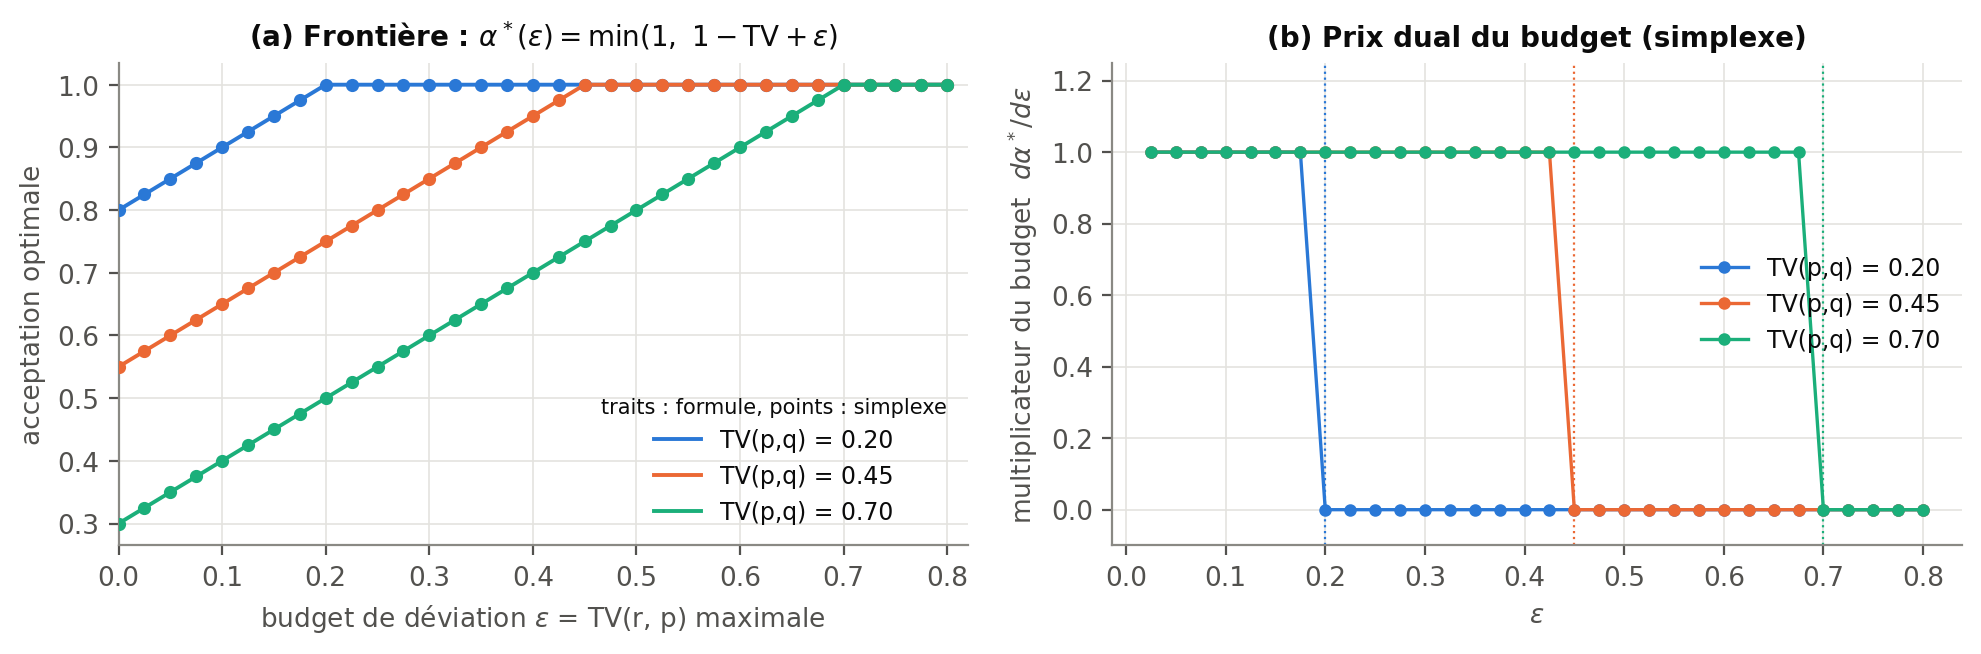
\includegraphics[width=\linewidth]{fig2_lossy_frontier.png}
\caption{(a) Acceptation optimale en fonction du budget $\varepsilon$, pour trois paires $(p,q)$ ; points : simplexe, traits : proposition~\ref{prop:perte} (écart maximal $2{,}8\times10^{-16}$). (b) Prix du budget $\kappa=-2\mu^*_B=d\alpha^*/d\varepsilon$ calculé à partir du dual renvoyé par le simplexe : 1 avant $\varepsilon=\TV$ (pointillés), 0 après.}
\label{fig:perte}
\end{figure}

%=====================================================================
\section{Partie II : répartir le budget entre les positions d'un bloc}
%=====================================================================
\subsection{Modèle : variables, objectif, contraintes}\label{sec:modeleII}
Un bloc compte $\gamma$ positions draftées. La position $t$ a une acceptation exacte $a_t=\beta(p_t,q_t)\in(0,1)$ et une \textbf{sensibilité} $s_t>0$ : la baisse de qualité de la réponse finale par unité de déviation (en variation totale) à cette position.

\paragraph{Variables :} les déviations $\varepsilon=(\varepsilon_1,\dots,\varepsilon_\gamma)$. \textbf{Hypothèses :}
\begin{itemize}
\item[(H1)] les acceptations des différentes positions sont indépendantes, comme dans~\cite{leviathan} ;
\item[(H2)] la perte de qualité est additive au premier ordre : $\sum_ts_t\varepsilon_t$ ;
\item[(H3)] d'après la proposition~\ref{prop:perte}, relâcher la position $t$ de $\varepsilon_t$ donne l'acceptation $\alpha_t=a_t+\varepsilon_t$, avec $0\le\varepsilon_t\le u_t:=1-a_t=\TV_t$ (au-delà, l'acceptation vaut déjà 1). On appelle $u_t$ la \emph{marge} de la position $t$.
\end{itemize}

\paragraph{Objectif : nombre moyen de tokens par passe du target.} Soit $N$ le nombre de tokens draftés acceptés dans le bloc. Le bloc s'arrête au premier rejet, donc « au moins $k$ acceptés » signifie « les $k$ premiers acceptés » et, sous (H1),
\[\Prob(N\ge k)=\alpha_1\alpha_2\cdots\alpha_k=:P_k\qquad(P_0=1).\]
Pour une variable à valeurs entières, $\Esp[N]=\sum_{k\ge1}\Prob(N\ge k)$. Le target émet en plus un token à la fin de chaque passe (sa correction en cas de rejet, ou un token bonus si tout est accepté). D'où
\[E(\varepsilon)=1+\Esp[N]=1+\sum_{k=1}^{\gamma}\prod_{j=1}^{k}(a_j+\varepsilon_j).\]
\textbf{Contraintes :} $K=\{\varepsilon\in\R^\gamma:\ 0\le\varepsilon_t\le u_t,\ s\cdot\varepsilon\le B\}$, toutes affines.
\[(Q_B)\qquad \max_{\varepsilon\in K}\ E(\varepsilon)\qquad\Longleftrightarrow\qquad \min_{\varepsilon\in K}\ J(\varepsilon)=-E(\varepsilon).\]
On le compare au \textbf{modèle A}, qui ignore la structure en bloc et maximise $\sum_t\alpha_t$ : un PL de type sac à dos fractionnaire.

\begin{exemple}[$\gamma=3$, sans relâchement, $a=(0{,}9;0{,}5;0{,}8)$]
$P_1=0{,}9$, $P_2=0{,}45$, $P_3=0{,}36$, donc $E=2{,}71$ tokens par passe. Le faible $a_2=0{,}5$ coupe la moitié des blocs à la position 2 : la position 3, pourtant facile, n'est atteinte qu'une fois sur deux.
\end{exemple}

\subsection{Existence, structure et unicité}\label{sec:existenceII}
\paragraph{Existence.} $K$ est un polyèdre non vide ($0\in K$ car $B\ge0$), fermé et borné ($0\le\varepsilon\le u$), donc compact ; $J=-E$ est un polynôme, donc continu. Le théorème~2.2.1 (la coercivité est automatique sur un borné) donne au moins un minimum de $J$, c'est-à-dire un maximum de $E$.

\paragraph{Gradient.} $\alpha_t$ n'apparaît que dans les $P_k$ avec $k\ge t$, et linéairement : $\partial P_k/\partial\alpha_t=P_k/\alpha_t$ pour $k\ge t$, $0$ sinon. Comme $\partial\alpha_t/\partial\varepsilon_t=1$,
\[\partial_tE=\sum_{k\ge t}\frac{P_k}{\alpha_t}=P_{t-1}\big(1+\alpha_{t+1}+\alpha_{t+1}\alpha_{t+2}+\dots+\alpha_{t+1}\cdots\alpha_\gamma\big)=P_{t-1}\,T_t,\]
où $P_{t-1}$ est la \textbf{probabilité d'atteindre} la position $t$ et $T_t$ (défini par $T_\gamma=1$, $T_t=1+\alpha_{t+1}T_{t+1}$) le \textbf{nombre de tokens} que l'acceptation de $t$ « débloque », elle comprise. Tous les $\alpha_j$ sont $>0$, donc $\partial_tE>0$ : $E$ croît strictement en chaque variable.

\paragraph{Hessienne.} $E$ est affine en chaque $\alpha_t$ séparément (fonction multilinéaire), donc $\partial^2_{tt}E=0$. Pour $i<j$, $\alpha_j$ n'apparaît que dans $T_i$, et
\[\partial^2_{ij}E=P_{i-1}\Big(\prod_{i<k<j}\alpha_k\Big)T_j\ >0.\]

\paragraph{Non-concavité.} La hessienne $H$ est symétrique, non nulle et de trace nulle : ses valeurs propres sont réelles, de somme nulle et pas toutes nulles, donc l'une est $>0$. $H$ n'est semi-définie négative en aucun point : $E$ \textbf{n'est pas concave} ($J$ n'est pas convexe).

\begin{exemple}[$\gamma=2$, $a=(0{,}5;0{,}5)$]
$E=1+\alpha_1+\alpha_1\alpha_2$, $\nabla E=(1+\alpha_2,\alpha_1)$ et $H=\begin{psmallmatrix}0&1\\1&0\end{psmallmatrix}$, de valeurs propres $\pm1$. Sur la diagonale $\varepsilon_1=\varepsilon_2$ : $E(0;0)=1{,}75$, $E(0{,}5;0{,}5)=3$, mais $E(0{,}25;0{,}25)=2{,}3125$, \emph{sous} la corde $(1{,}75+3)/2=2{,}375$ ; une fonction concave serait au-dessus.
\end{exemple}

\paragraph{Lecture.} $\partial^2_{ij}E>0$ signifie que relâcher une position augmente la valeur marginale des autres (on atteint plus souvent les suivantes) : les positions sont \textbf{complémentaires}. Conséquence : les résultats d'unicité par convexité (Prop.~2.3.4, Th.~2.3.8) ne s'appliquent pas, et l'on ne peut pas exclure a priori plusieurs maxima locaux.

\begin{lemme}[concavité le long des échanges]\label{lem:echange}
Pour deux positions $i\ne j$, la direction $d=s_je_i-s_ie_j$ conserve le coût ($s\cdot d=0$), et $h\mapsto E(\varepsilon+hd)$ est un trinôme strictement concave.
\end{lemme}
\begin{proof}
À coordonnées autres que $i,j$ fixées, $E$ est affine en $\alpha_i$ et en $\alpha_j$ séparément : $E=c_0+c_i\alpha_i+c_j\alpha_j+\partial^2_{ij}E\,\alpha_i\alpha_j$, où $\partial^2_{ij}E>0$ ne dépend ni de $\alpha_i$ ni de $\alpha_j$. Le long de $d$, $\alpha_i\leftarrow\alpha_i+hs_j$ et $\alpha_j\leftarrow\alpha_j-hs_i$ : le coefficient de $h^2$ vaut $-s_is_j\,\partial^2_{ij}E<0$.
\end{proof}
Transférer du budget d'une position à une autre est donc toujours un problème concave en dimension~1 : la non-concavité de $E$ vient des directions qui font varier deux positions dans le même sens (comme $\varepsilon_1=\varepsilon_2$ dans l'exemple) ou plus de deux positions à la fois. Ce lemme explique la proposition~\ref{prop:gamma2} ci-dessous et rend plausible l'unimodalité observée au §\ref{sec:algoII}, sans la démontrer pour $\gamma\ge3$.

\begin{lemme}[budget saturé]\label{lem:sature}
En tout maximum local, ou bien $s\cdot\varepsilon=B$, ou bien $\varepsilon=u$ (budget surabondant, $B\ge s\cdot u$).
\end{lemme}
\begin{proof}
Si $s\cdot\varepsilon<B$ et $\varepsilon_t<u_t$ pour un $t$, alors $\varepsilon+he_t\in K$ pour $h>0$ petit, et $E(\varepsilon+he_t)=E(\varepsilon)+h\,\partial_tE+o(h)>E(\varepsilon)$ puisque $\partial_tE>0$ : ce n'est pas un maximum local.
\end{proof}

\begin{proposition}[cas $\gamma=2$ : unicité et solution explicite]\label{prop:gamma2}
Si $B<s\cdot u$, le maximum est unique. On note $\kappa_s=s_1/s_2$ et $c=a_2+B/s_2$. Avec $\eta^*=\tfrac12\big((1+c)/\kappa_s-a_1\big)$, la solution est $\varepsilon_1^*=\mathrm{proj}_{[\eta_-,\eta_+]}(\eta^*)$ et $\varepsilon_2^*=(B-s_1\varepsilon_1^*)/s_2$, où $[\eta_-,\eta_+]=\big[\max\big(0,(B-s_2u_2)/s_1\big),\ \min\big(u_1,B/s_1\big)\big]$ est l'ensemble des $\varepsilon_1$ compatibles avec les bornes. Si $\eta_-<\eta^*<\eta_+$, la valeur optimale et le multiplicateur valent
\[E^*(B)=1+\frac{(1+c+\kappa_sa_1)^2}{4\kappa_s},\qquad \lambda^*=\frac{1+c+\kappa_sa_1}{2s_1}=\frac{dE^*}{dB}.\]
\end{proposition}
\begin{proof}
Par le lemme~\ref{lem:sature}, tout maximum est sur le segment $\{s\cdot\varepsilon=B\}\cap K$. On pose $\varepsilon_1=\eta$, $\varepsilon_2=(B-s_1\eta)/s_2$, soit $\alpha_1=a_1+\eta$ et $\alpha_2=c-\kappa_s\eta$ ; les bornes imposent $\eta\in[\eta_-,\eta_+]$. Alors
\[E(\eta)=1+(a_1+\eta)(1+c-\kappa_s\eta),\qquad E'(\eta)=(1+c)-\kappa_s(a_1+2\eta),\qquad E''(\eta)=-2\kappa_s<0.\]
$E$ est un trinôme strictement concave (c'est le lemme~\ref{lem:echange}) : son maximum sur un segment est unique, égal à $\eta^*$ (zéro de $E'$) projeté sur $[\eta_-,\eta_+]$. Si $\eta^*$ est intérieur, $a_1+\eta^*=(1+c+\kappa_sa_1)/(2\kappa_s)$ et $1+c-\kappa_s\eta^*=(1+c+\kappa_sa_1)/2$, d'où $E^*$. Enfin $c$ dépend de $B$ avec $dc/dB=1/s_2$, donc $dE^*/dB=(1+c+\kappa_sa_1)/(2\kappa_ss_2)=(1+\alpha_2^*)/s_1=\partial_1E/s_1=\lambda^*$ (§\ref{sec:kkt}).
\end{proof}
Dans ce régime, $E^*(B)$ est un polynôme de degré 2 en $B$, de coefficient dominant positif : la frontière est \emph{convexe} et le prix $\lambda^*$ croît avec $B$.

\begin{exemple}[instance de la figure~\ref{fig:paysage}]
$a=(0{,}55;0{,}7)$, $s=(1{,}5;0{,}6)$, $B=0{,}35\,s\cdot u=0{,}29925$.
\begin{itemize}
\item $c=0{,}7+0{,}29925/0{,}6=1{,}19875$, $\kappa_s=2{,}5$ ; $\varepsilon_1^*=\tfrac12(0{,}4\times2{,}19875-0{,}55)=0{,}16475\in[\eta_-,\eta_+]=[0{,}0795;0{,}1995]$ ; $\varepsilon_2^*=(0{,}29925-1{,}5\times0{,}16475)/0{,}6=0{,}086875$.
\item $\alpha^*=(0{,}71475;0{,}786875)$ et $E^*=1+0{,}71475\times1{,}786875=2{,}2772$.
\item KKT : $\nabla E=(1+\alpha_2,\alpha_1)=(1{,}786875;0{,}71475)$ et $\partial_1E/s_1=1{,}19125=\partial_2E/s_2$ : $\nabla E=\lambda s$ avec $\lambda=1{,}19125$, qui est aussi la valeur de $dE^*/dB$ donnée par la proposition.
\item Le gradient projeté trouve exactement ces valeurs. Le modèle A relâche d'abord la position la moins sensible (la 2), sature $\varepsilon_2=u_2=0{,}3$ puis $\varepsilon_1=0{,}0795$ : $E=2{,}2590$ contre $2{,}2772$.
\end{itemize}
\end{exemple}

\begin{proposition}[positions identiques : relâcher d'abord le début]\label{prop:ordre}
Si $a_t\equiv a$ et $s_t\equiv s$, toute solution optimale vérifie $\alpha_1\ge\alpha_2\ge\dots\ge\alpha_\gamma$.
\end{proposition}
\begin{proof}
Supposons $\alpha_t<\alpha_{t+1}$ en un optimum et échangeons $\varepsilon_t$ et $\varepsilon_{t+1}$. Le point obtenu est admissible (mêmes marges, même coût). Pour $k<t$, $P_k$ ne contient ni $\alpha_t$ ni $\alpha_{t+1}$ ; pour $k\ge t+1$, il contient le produit $\alpha_t\alpha_{t+1}$, inchangé. Seul $P_t=P_{t-1}\alpha_t$ change et devient $P_{t-1}\alpha_{t+1}$ : $E$ augmente de $P_{t-1}(\alpha_{t+1}-\alpha_t)>0$, ce qui contredit l'optimalité.
\end{proof}

\begin{figure}[htbp]
\centering
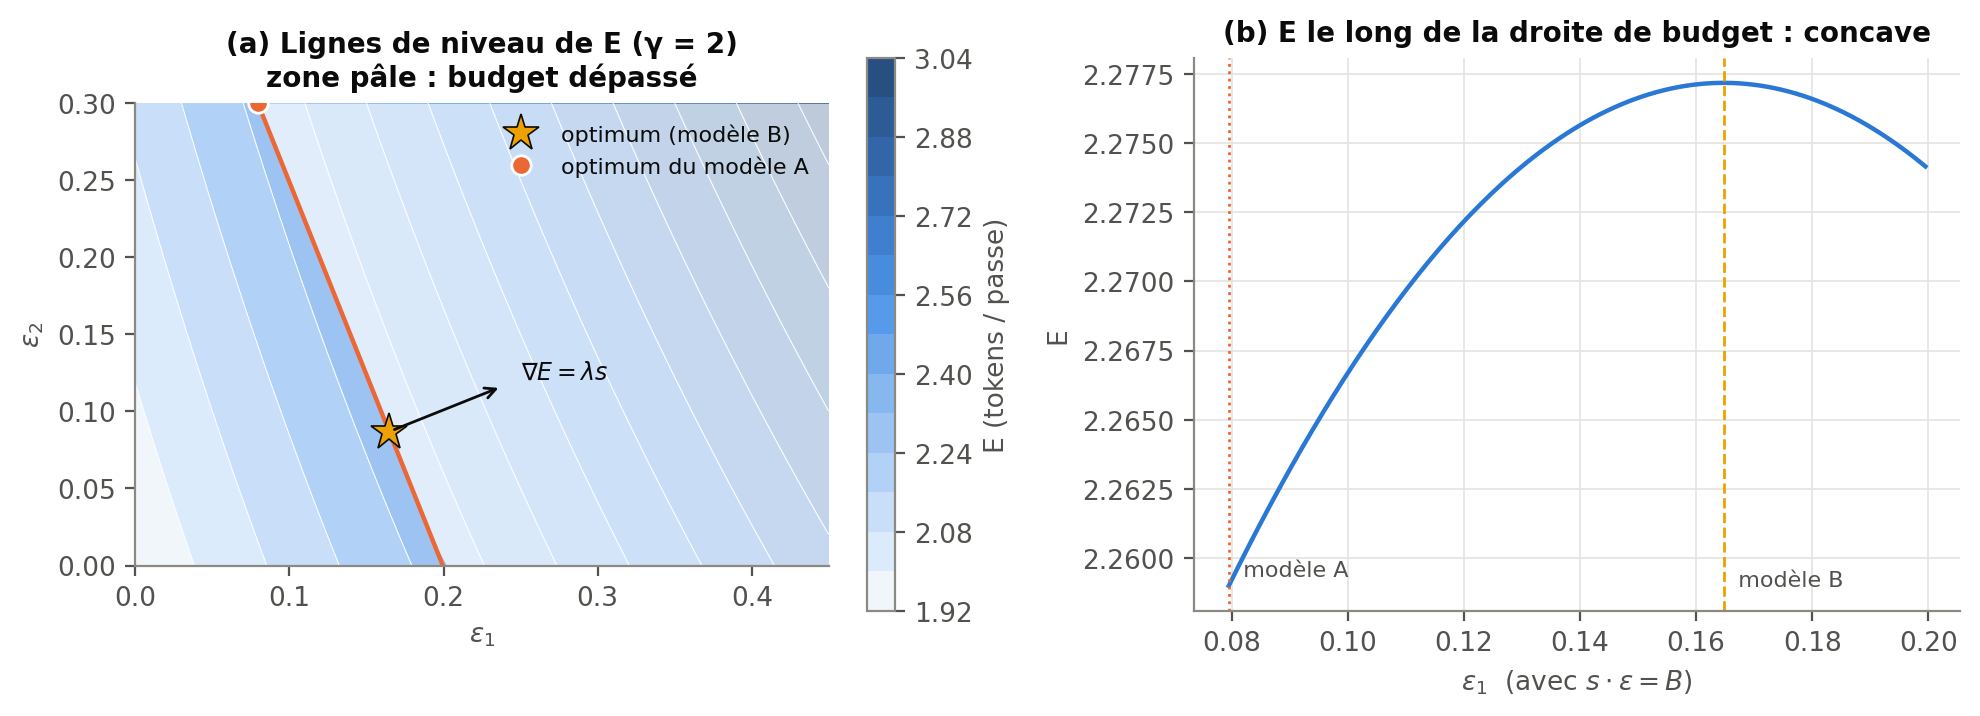
\includegraphics[width=\linewidth]{fig3_landscape_gamma2.png}
\caption{$\gamma=2$, $a=(0{,}55;0{,}7)$, $s=(1{,}5;0{,}6)$, $B=0{,}35\,s\cdot u$. (a) À l'optimum, $\nabla E$ est orthogonal à la droite de budget ($\nabla E=\lambda s$). (b) Le long de cette droite, $E$ est un trinôme concave ($E''=-2s_1/s_2=-5$). Le modèle A choisit le bord ($E=2{,}2590$ contre $2{,}2772$).}
\label{fig:paysage}
\end{figure}

\subsection{Conditions d'optimalité (KKT)}\label{sec:kkt}
\paragraph{Contraintes écrites $F_i(\varepsilon)\le0$ et leurs gradients.}
\begin{center}
\small
\begin{tabular}{@{}llll@{}}
\toprule
Contrainte & $F_i(\varepsilon)$ & $\nabla F_i$ & Multiplicateur\\\midrule
budget & $s\cdot\varepsilon-B$ & $s$ & $\lambda\ge0$\\
borne basse, position $t$ & $-\varepsilon_t$ & $-e_t$ & $\mu^0_t\ge0$\\
borne haute, position $t$ & $\varepsilon_t-u_t$ & $e_t$ & $\mu^1_t\ge0$\\
\bottomrule
\end{tabular}
\end{center}

\paragraph{Qualification.} Toutes les $F_i$ sont affines. La définition~2.5.15 demande une direction $w$ telle que $\sca{\nabla F_i}{w}<0$ pour chaque contrainte active, l'égalité $\sca{\nabla F_i}{w}=0$ étant permise pour les contraintes affines : $w=0$ convient (Rq.~2.5.16). Les contraintes sont qualifiées en tout point de $K$.

\paragraph{Conditions KKT} (Th.~2.5.17, appliqué à $J=-E$). En tout minimum local de $J$ (maximum local de $E$), il existe $\lambda,\mu^0,\mu^1\ge0$ tels que
\[\nabla J+\lambda s-\sum_t\mu^0_te_t+\sum_t\mu^1_te_t=0\quad\Longleftrightarrow\quad \nabla E(\varepsilon)=\lambda s-\mu^0+\mu^1,\]
avec les écarts complémentaires $\lambda(s\cdot\varepsilon-B)=0$, $\mu^0_t\varepsilon_t=0$ et $\mu^1_t(u_t-\varepsilon_t)=0$.
Ces conditions sont \textbf{seulement nécessaires} : $J$ n'est pas convexe, donc le théorème de Kuhn--Tucker (Th.~2.6.4), qui les rendrait suffisantes, ne s'applique pas. Un point KKT peut a priori être un maximum local non global, ou un point selle.

\paragraph{Lecture coordonnée par coordonnée.} Notons $\rho_t=\partial_tE/s_t$ le \textbf{rendement} de la position $t$ (tokens gagnés par unité de qualité perdue). La $t$-ième équation s'écrit $\partial_tE=\lambda s_t-\mu^0_t+\mu^1_t$ :
\begin{itemize}
\item si $0<\varepsilon_t<u_t$, aucune borne n'est active : $\mu^0_t=\mu^1_t=0$ et $\rho_t=\lambda$ ;
\item si $\varepsilon_t=0$ : $\mu^1_t=0$, donc $\rho_t\le\lambda$ (pas rentable, on ne relâche pas) ;
\item si $\varepsilon_t=u_t$ : $\mu^0_t=0$, donc $\rho_t\ge\lambda$ (très rentable, on relâche au maximum).
\end{itemize}
C'est une \textbf{règle de seuil} : on relâche les positions dont le rendement dépasse le prix $\lambda$.
\begin{itemize}
\item \textbf{Modèle A} : $\partial_t(\sum_j\alpha_j)=1$, donc $\rho_t=1/s_t$ ne dépend pas de $\varepsilon$. On trie par sensibilité croissante et l'on sature les positions dans cet ordre jusqu'à épuisement du budget ; $\lambda=1/s_{t^*}$ pour la position charnière $t^*$ (sac à dos fractionnaire). Notre simplexe et cet algorithme glouton donnent la même solution (tests unitaires).
\item \textbf{Modèle B} : $\rho_t=P_{t-1}T_t/s_t$ dépend de la \textbf{place} de la position : une position précoce est atteinte souvent ($P_{t-1}$ grand) et débloque beaucoup de tokens ($T_t$ grand). C'est pourquoi le budget va au début du bloc.
\end{itemize}

\paragraph{$\lambda$ est le prix marginal du budget.} Soit $\varepsilon^*$ optimal pour le budget $B$, avec une position intérieure $t$ ($0<\varepsilon^*_t<u_t$), et soit $0<h\le s_t\min(\varepsilon^*_t,u_t-\varepsilon^*_t)$. Le point $\varepsilon^*+(h/s_t)e_t$ est admissible pour le budget $B+h$, et $\varepsilon^*-(h/s_t)e_t$ pour le budget $B-h$. Comme $E$ est affine en $\varepsilon_t$ ($\partial^2_{tt}E=0$), $E$ y vaut exactement $E^*(B)\pm\partial_tE\,h/s_t=E^*(B)\pm\lambda h$. Donc $E^*(B+h)\ge E^*(B)+\lambda h$ et $E^*(B-h)\ge E^*(B)-\lambda h$, c'est-à-dire
\begin{equation}\label{eq:encadrement}
\frac{E^*(B)-E^*(B-h)}{h}\ \le\ \lambda\ \le\ \frac{E^*(B+h)-E^*(B)}{h}.
\end{equation}
Là où $E^*$ est dérivable, $\lambda=dE^*/dB$. C'est l'analogue du lemme~2.6.6 du cours, qui suppose la convexité ; ici, la structure multilinéaire de $E$ suffit. On le retrouve pour $\gamma=2$ (proposition~\ref{prop:gamma2}) et numériquement en S2, à 0,5\,\% près (figure~\ref{fig:frontiere}c).

\subsection{Algorithme : gradient projeté, et question des maxima locaux}\label{sec:algoII}
$K$ est convexe et la projection sur $K$ se calcule presque explicitement : on choisit le \textbf{gradient projeté} du cours, en montée,
\[\varepsilon_{k+1}=P_K\big(\varepsilon_k+\tau\nabla E(\varepsilon_k)\big).\]

\paragraph{1. Calcul de la projection $z=P_K(y)$.} C'est la solution de $\min_{z\in K}\tfrac12\nr{z-y}^2$, fonction fortement convexe : elle existe et est unique (Th.~2.3.8). On dualise seulement la contrainte de budget, avec un multiplicateur $\nu\ge0$ :
\[\min_{0\le z\le u}\ \tfrac12\nr{z-y}^2+\nu(s\cdot z-B)=\sum_t\Big[\tfrac12(z_t-y_t)^2+\nu s_tz_t\Big]-\nu B.\]
Le problème se sépare coordonnée par coordonnée : chaque terme est une parabole de minimum libre en $y_t-\nu s_t$, et sur $[0,u_t]$ le minimum est ce point ramené dans l'intervalle :
\[z_t(\nu)=\clip(y_t-\nu s_t,\ 0,\ u_t).\]
Si $s\cdot z(0)\le B$, on prend $\nu=0$. Sinon, $\Phi(\nu)=s\cdot z(\nu)$ est continue et décroissante, $\Phi(0)>B$ et $\Phi(\nu)=0\le B$ pour $\nu$ grand : le théorème des valeurs intermédiaires donne $\nu$ tel que $\Phi(\nu)=B$, calculé par dichotomie.
Dans les deux cas, $(z(\nu),\nu)$ vérifie les conditions KKT du problème de projection, avec le multiplicateur $\nu\ge0$ du budget ($\nu(s\cdot z(\nu)-B)=0$) et les multiplicateurs $\omega^0_t=(\nu s_t-y_t)_+$ et $\omega^1_t=(y_t-\nu s_t-u_t)_+$ des bornes : dans chacun des trois cas du clip, on vérifie $z_t-y_t+\nu s_t-\omega^0_t+\omega^1_t=0$ et les écarts complémentaires. Ce problème étant convexe à contraintes affines, ces conditions sont suffisantes (Th.~2.6.4) : $z(\nu)=P_K(y)$. C'est un problème dual de dimension~1.

\paragraph{2. Choix du pas.} Sur $K$, on a $\alpha\in[0,1]^\gamma$, donc $P_{i-1}\le1$, $\prod\alpha_k\le1$ et $T_j\le\gamma-j+1$ (somme de $\gamma-j+1$ produits $\le1$). D'où $|\partial^2_{ij}E|\le\gamma-\max(i,j)+1$ et, puisque $\nr{H}_2\le\nr{H}_F$,
\[\nr{\nabla E(x)-\nabla E(y)}\le L\nr{x-y}\quad(x,y\in K),\qquad L=\Big(\sum_{i\ne j}\big(\gamma-\max(i,j)+1\big)^2\Big)^{1/2}.\]
Pour $\gamma=2$, $L=\sqrt2$ (la vraie norme de $H$ vaut 1) ; pour $\gamma=8$, $L\approx25{,}9$. On prend $\tau=1/L$.

\paragraph{3. Convergence.} Le théorème~3.4.1 suppose $J$ $\alpha$-convexe : il \textbf{ne s'applique pas} ici, et pour la même raison ni Uzawa (Th.~3.4.3) ni la pénalisation (Prop.~3.4.6). On démontre en annexe~\ref{app:convergence}, avec l'inéquation d'Euler (Th.~2.5.1), que $E(\varepsilon_k)$ croît, que les pas tendent vers 0 et que toute valeur d'adhérence de $(\varepsilon_k)$ vérifie les conditions KKT. Pour un problème non concave, c'est la meilleure garantie générale : un point KKT n'est pas forcément un maximum global.

\paragraph{4. Global ou local ?} On lance le gradient projeté depuis 20 points initiaux aléatoires sur 100 instances aléatoires ($\gamma\in\{3,4,6,8\}$ ; la hessienne y est indéfinie, comme en tout point d'après le §\ref{sec:existenceII}). L'écart maximal entre valeurs finales vaut $1{,}8\times10^{-15}$, l'écart maximal entre solutions $1{,}1\times10^{-8}$, et le résidu KKT maximal $2{,}9\times10^{-10}$. Nous n'avons donc \textbf{jamais observé deux maxima locaux distincts} : le problème est non concave mais, empiriquement, unimodal. L'unicité n'est démontrée que pour $\gamma=2$ (proposition~\ref{prop:gamma2}).

\begin{figure}[htbp]
\centering
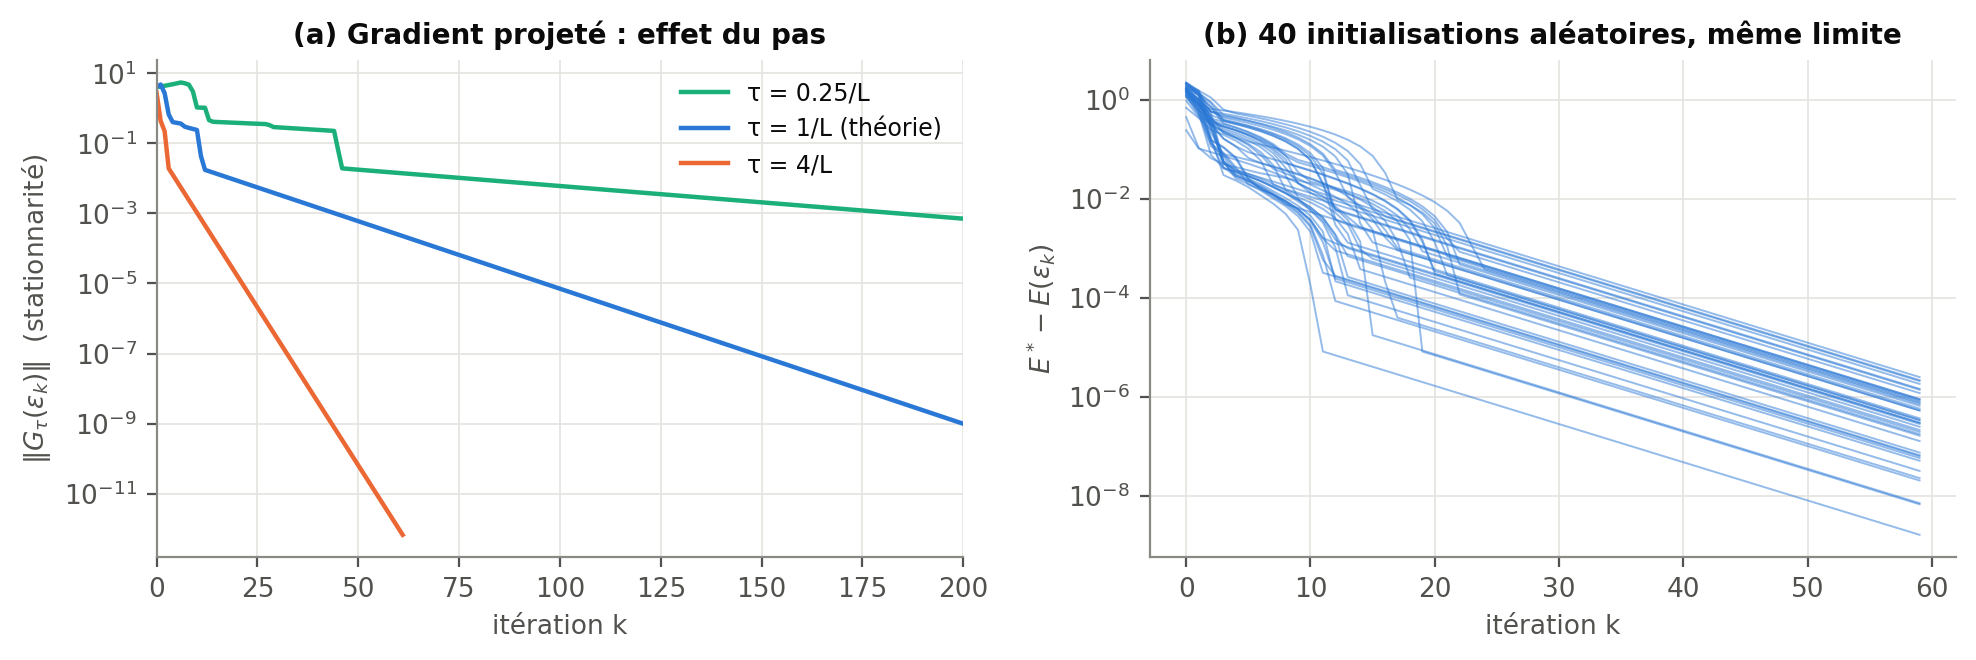
\includegraphics[width=\linewidth]{fig4_convergence.png}
\caption{Instance $\gamma=8$. (a) Norme de l'application gradient $\nr{P_K(\varepsilon+\tau\nabla E)-\varepsilon}/\tau$ pour trois pas : convergence linéaire. Avec $\tau=1/L$, 279 itérations ; avec $\tau=4/L$, 62 itérations (la monotonie est observée mais n'est plus garantie, voir l'annexe~\ref{app:convergence}) ; $\tau=0{,}25/L$ est beaucoup plus lent. (b) 40 départs aléatoires convergent vers la même valeur $E^*=5{,}4544$.}
\label{fig:convergence}
\end{figure}

\subsection{Résultats : où placer la déviation ?}\label{sec:resultats}
On prend $\gamma=6$, $a_t=0{,}6$ et un budget $B=0{,}3\,B_{\max}$ (où $B_{\max}=s\cdot u$), avec trois profils de sensibilité (figure~\ref{fig:allocation}).
\begin{itemize}
\item \textbf{S1 (positions identiques, $s_t=1$).} Le modèle B relâche dans l'ordre $1,2,\dots$ (proposition~\ref{prop:ordre}). Le modèle A est \emph{indifférent} : tous les $\rho_t=1/s$ sont égaux, donc toute répartition de même coût est A-optimale, y compris « fin d'abord », qui ne donne que $E=2{,}54$ contre $4{,}12$. La solution gloutonne de A coïncide ici avec B uniquement grâce à son départage par indice.
\item \textbf{S2 (début plus sensible, $s=(2;1{,}7;1{,}4;1{,}1;0{,}8;0{,}5)$).} Le modèle A relâche les dernières positions, les moins chères. Le modèle B relâche malgré tout les \textbf{premières} : $E=3{,}52$ contre $2{,}79$ pour A ($+26\,\%$) et $3{,}21$ pour une déviation uniforme. À l'optimum, $\rho_1=\rho_2=\lambda=1{,}308$ (positions intérieures) et $\rho_t<\lambda$ ailleurs, comme le prévoit KKT.
\item \textbf{S3 (deux tokens pivots, $s=2{,}5$ en positions 2 et 5, $0{,}3$ ailleurs).} Le modèle B évite le pivot tardif (position 5) mais relâche en partie le pivot précoce (position 2), qui conditionne l'accès aux positions 3 et 4. L'écart avec A est faible ($4{,}98$ contre $4{,}96$).
\end{itemize}

\begin{figure}[htbp]
\centering
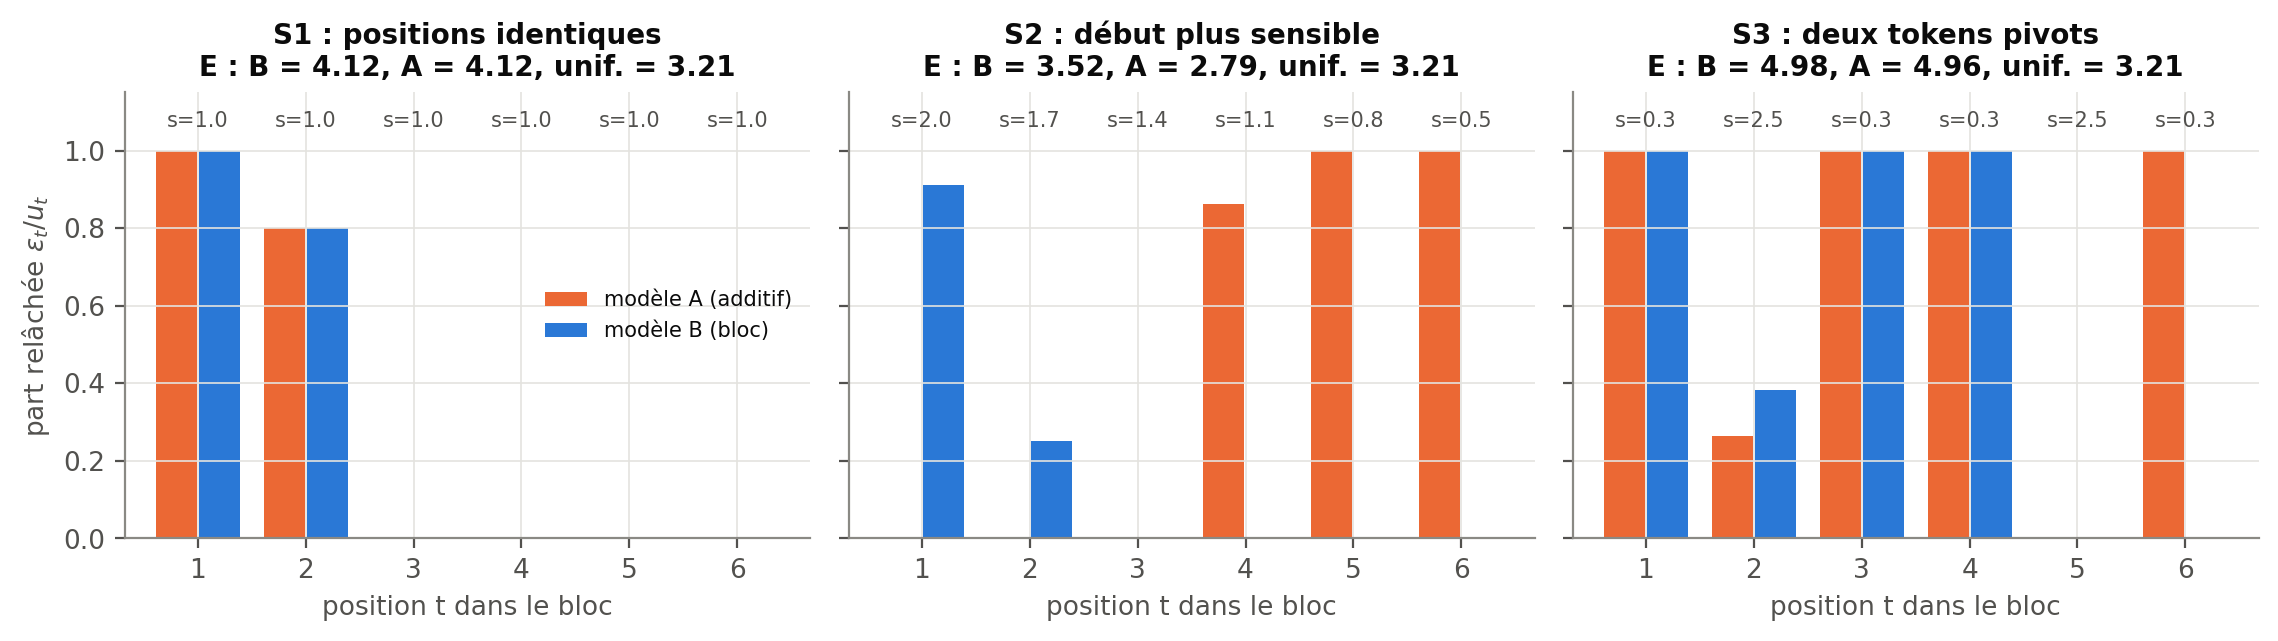
\includegraphics[width=\linewidth]{fig5_allocation.png}
\caption{Part relâchée $\varepsilon_t/u_t$ par position, pour le modèle additif A (orange) et le modèle par blocs B (bleu). Les sensibilités $s_t$ sont indiquées au-dessus de chaque position.}
\label{fig:allocation}
\end{figure}

\paragraph{Frontière vitesse--budget (figure~\ref{fig:frontiere}).} Pour chaque budget, on compare l'optimum aux heuristiques. En S2, le gain maximal sur A vaut 0,97 token par passe, et sur la déviation uniforme 0,40. L'heuristique « fin d'abord » relâche le moins les premiers tokens, à la manière de~\cite{secure} qui vérifie plus strictement le début pour la sécurité ; du point de vue de la vitesse, elle est toujours la pire (à égalité avec A en S2).

La forme de la frontière $E^*(B)$ dépend du profil. En \textbf{S2}, elle est convexe et $\lambda^*(B)$ croît (figure~\ref{fig:frontiere}c) : l'effet de complémentarité des positions ($\partial^2_{ij}E>0$) domine, et il vaut mieux concentrer la déviation sur quelques positions que de la diluer (seules les deux premières sont relâchées, figure~\ref{fig:allocation}). En \textbf{S3}, au contraire, la frontière est essentiellement concave (figure~\ref{fig:frontiere}b) : sa pente décroît d'un segment à l'autre, car on dépense d'abord sur les positions bon marché ($s_t=0{,}3$), très rentables, puis sur les pivots, chers, comme dans un sac à dos. Les deux effets coexistent : en général, $E^*(B)$ n'est ni convexe ni concave.

L'encadrement~\eqref{eq:encadrement} dit où la pente peut baisser. Pour $B<s\cdot u$, le budget est saturé (lemme~\ref{lem:sature}). Si de plus $B$ n'est pas l'une des valeurs « sommets » $B_I=\sum_{t\in I}s_tu_t$ ($I\subset\{1,\dots,\gamma\}$), l'optimum n'est pas un sommet du pavé : il a une position intérieure, et \eqref{eq:encadrement} donne en $B$ une droite d'appui locale de pente $\lambda$, située sous $E^*$. Or une fonction continue qui admet une telle droite en tout point d'un intervalle est convexe sur cet intervalle\footnote{Si $f$ passait strictement au-dessus d'une de ses cordes sur $[c,d]$, la différence $g$ entre $f$ et la corde atteindrait un maximum $>0$ en un $x_0\in\,]c,d[$. La droite d'appui en $x_0$ a forcément la pente de la corde (sinon $g$ dépasserait $g(x_0)$ d'un côté de $x_0$), donc $g=g(x_0)$ près de $x_0$ : l'ensemble où $g$ atteint son maximum serait non vide, ouvert et fermé dans $[c,d]$, sans contenir $c$ ni $d$, ce qui contredit la connexité. $E^*$ est bien continue, et même localement lipschitzienne : si $\varepsilon'$ est optimal pour $B'>B>0$, le point $(B/B')\varepsilon'$ est admissible pour $B$.}. Ainsi, \textbf{$E^*$ est convexe entre deux valeurs $B_I$ consécutives, et sa pente ne peut baisser qu'en un $B_I$}. En S3, l'optimum relâche l'une après l'autre les positions bon marché 1, 3 et 4, puis le pivot précoce 2 (un temps avec la position 6), et le pivot tardif 5 en dernier : la pente chute en $B_I$ pour $I=\{1\}$, $\{1,3\}$, $\{1,3,4\}$ et $\{1,2,3,4,6\}$, d'où l'allure concave. Pour $\gamma=2$, en régime intérieur, $E^*$ est convexe (proposition~\ref{prop:gamma2}).

\begin{figure}[htbp]
\centering
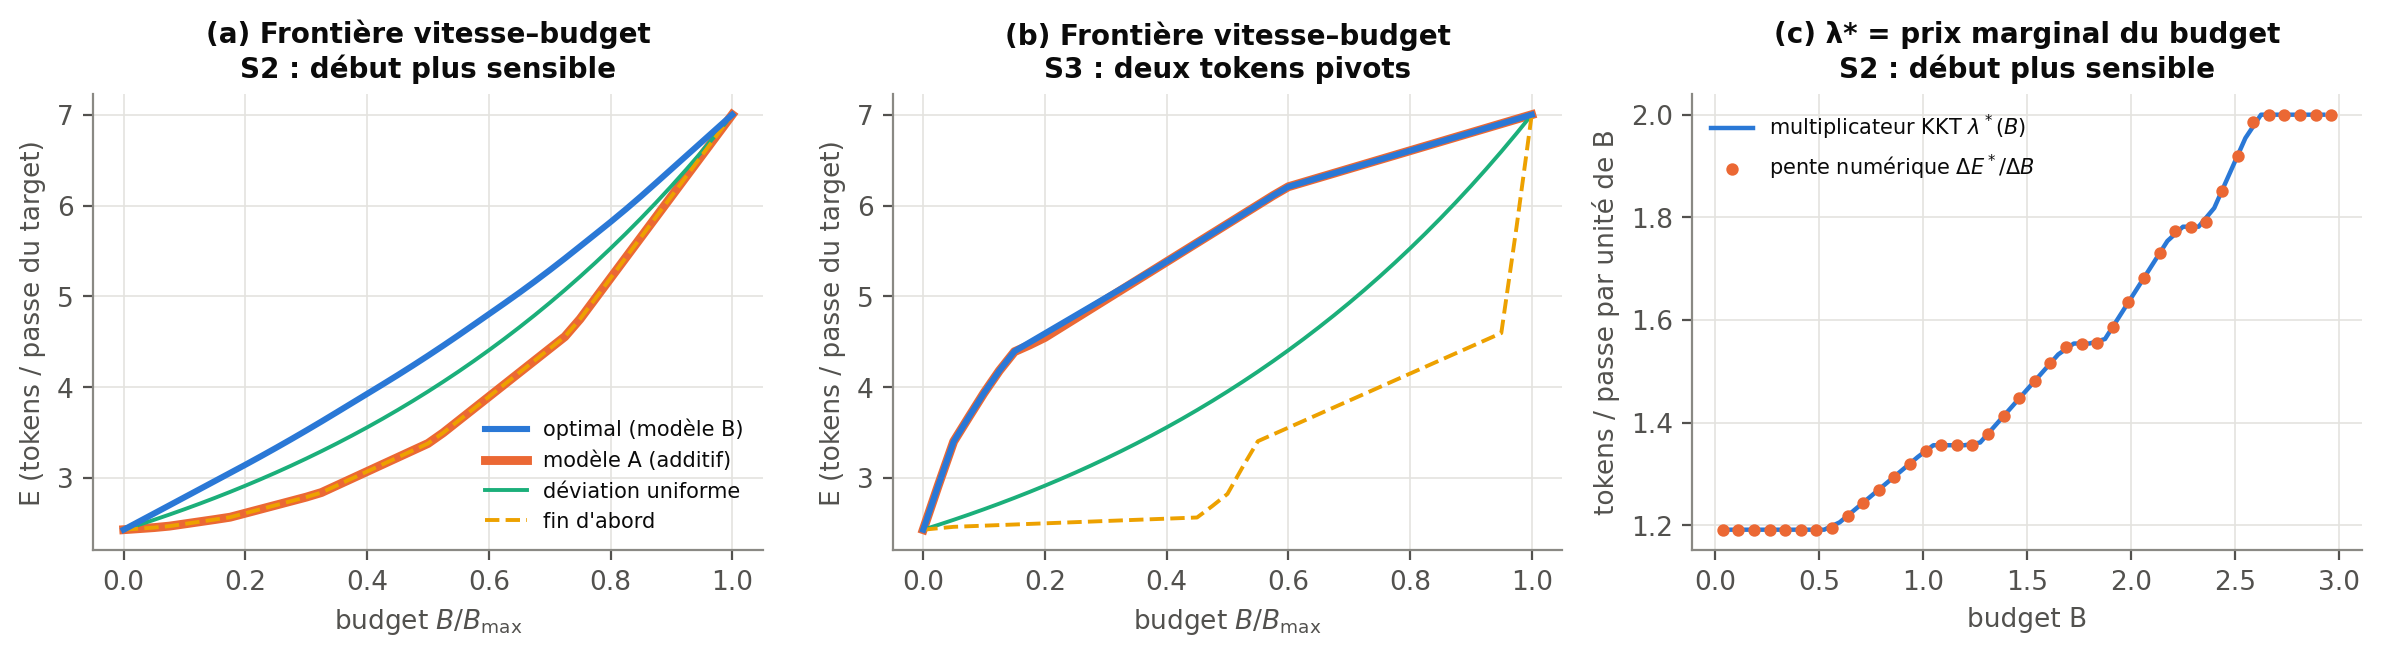
\includegraphics[width=\linewidth]{fig6_frontier.png}
\caption{(a-b) Nombre moyen de tokens par passe du target en fonction du budget, pour l'allocation optimale et trois heuristiques. (c) Multiplicateur KKT $\lambda^*(B)$ et pente numérique $\Delta E^*/\Delta B$ en S2 : le multiplicateur est bien le prix marginal du budget.}
\label{fig:frontiere}
\end{figure}

%=====================================================================
\section{Données réelles : Qwen2.5-1.5B (target) et Qwen2.5-0.5B (draft) sur GSM8K}\label{sec:reel}
%=====================================================================
Le target rédige des solutions à 16 problèmes GSM8K tirés au hasard, en décodage glouton (2344 tokens générés), tronquées à 150 tokens : seules les lois $(p_t,q_t)$ comptent ici, pas la justesse des réponses. À chaque position, on calcule $a_t=\beta(p_t,q_t)$ sur le vocabulaire complet. L'acceptation exacte moyenne vaut 0,893 (figure~\ref{fig:reel}a), et 47\,\% des positions ont $a_t>0{,}99$ ; elle vaut 0,982 sur les tokens contenant un chiffre (15\,\% des tokens), contre 0,878 sur les autres.
Les sensibilités ne sont \textbf{pas mesurées} dans ce DM (c'est l'objet du projet de recherche). On utilise un proxy explicite : $s_t=10$ si le token contient un chiffre, $s_t=1$ sinon (les nombres décident de la réponse à GSM8K).
On découpe la séquence en blocs consécutifs de $\gamma=5$ et l'on maximise $\sum_{\text{blocs}}E$ sous un budget commun ; le même gradient projeté s'applique, car la hessienne est diagonale par blocs.
\begin{itemize}
\item Sans relâchement, on obtient 4,66 tokens par passe et par bloc, et 6,00 si l'on relâche tout. À $B=0{,}2\,B_{\max}$ : 5,18 (optimal), 4,98 (modèle A), 4,87 (uniforme).
\item Le gain maximal de l'allocation optimale vaut 0,235 token par passe sur A et 0,467 sur l'uniforme (figure~\ref{fig:reel}b). Il est plus faible qu'en synthétique, parce que la plupart des positions réelles ont déjà $a_t\approx1$.
\item L'optimum ne dépense \textbf{rien} sur les tokens numériques tant que $B\le0{,}75\,B_{\max}$ : ils sont à la fois chers ($s_t=10$) et déjà presque toujours acceptés (les nombres sont souvent recopiés de l'énoncé).
\item À $B=0{,}2\,B_{\max}$, l'optimum relâche la première position du bloc à 73\,\% de sa marge, la deuxième à 43\,\%, et les suivantes à 0\,\% ; le modèle A ne distingue pas les positions (entre 22 et 28\,\%, figure~\ref{fig:reel}c). On retrouve sur données réelles la conclusion de la partie II : la déviation doit aller au \textbf{début} du bloc.
\end{itemize}

\begin{figure}[htbp]
\centering
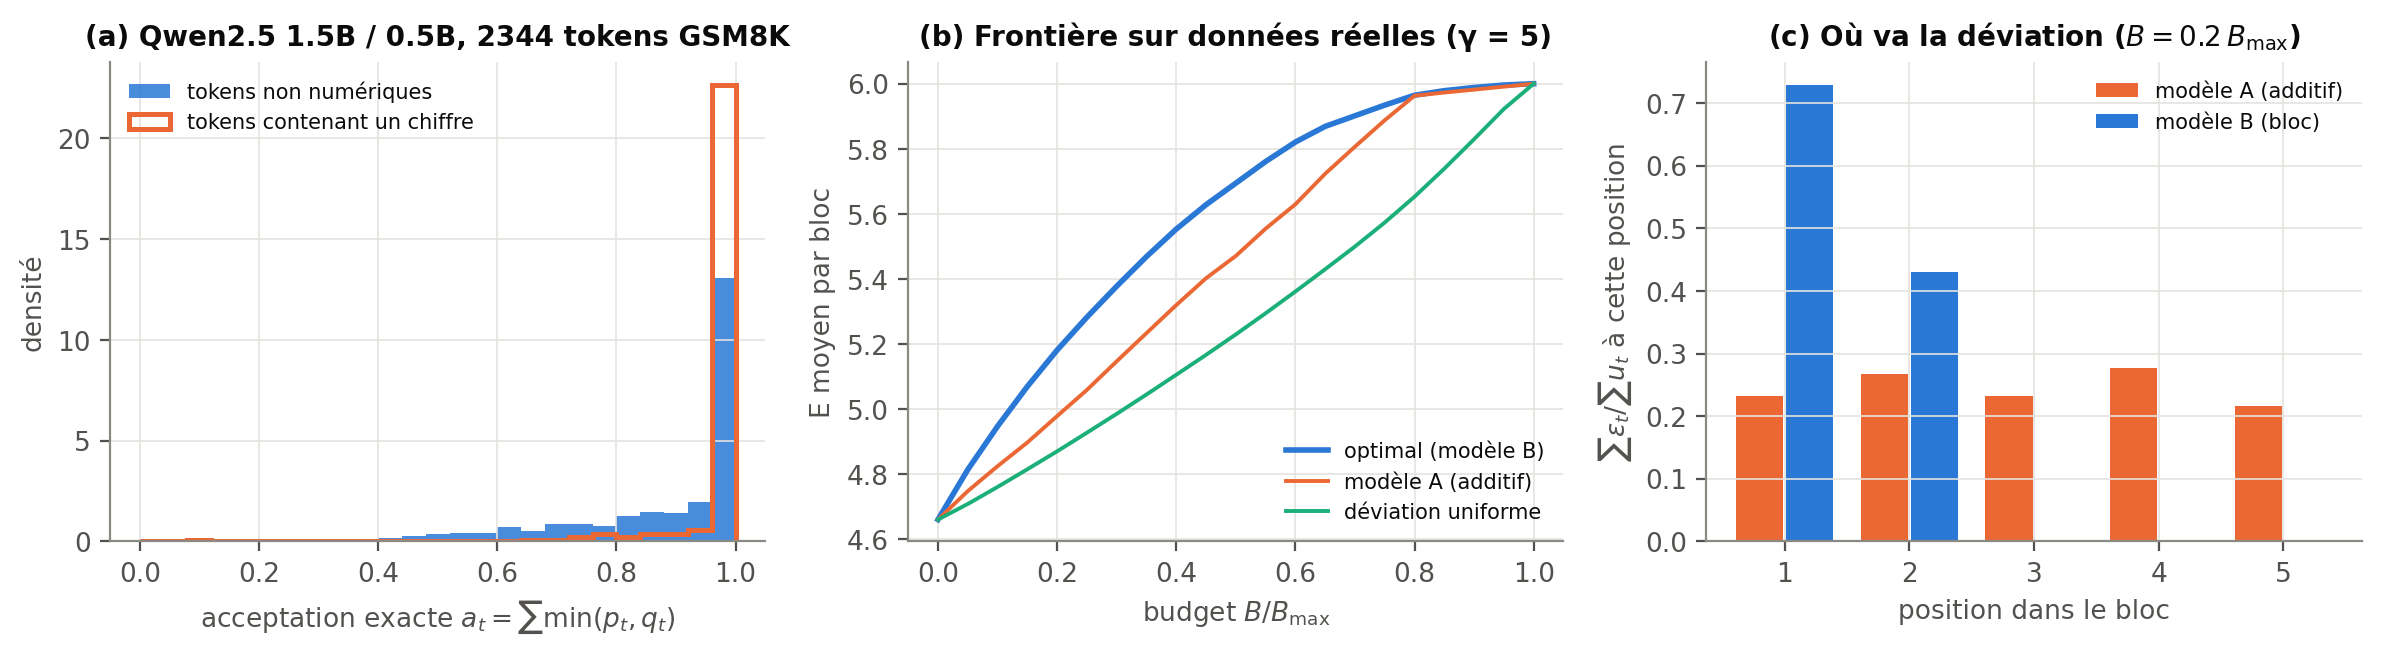
\includegraphics[width=\linewidth]{fig7_real_data.png}
\caption{(a) Distribution des acceptations exactes mesurées. (b) Frontière vitesse--budget sur les données réelles. (c) Part relâchée selon la position dans le bloc, à $B=0{,}2\,B_{\max}$.}
\label{fig:reel}
\end{figure}

%=====================================================================
\section{Conclusion, limites et lien avec le projet}
%=====================================================================
Les deux problèmes se traitent avec les outils du cours. La partie I est un PL de transport : le simplexe et la dualité en donnent la valeur ($1-\TV$), un certificat explicite et le prix exact d'une unité de déviation. La partie II est un problème non concave sous contraintes affines : les contraintes y sont qualifiées, les conditions KKT donnent une règle de seuil interprétable, dont le seuil $\lambda$ est le prix marginal exact du budget (même sans concavité), le gradient projeté converge vers un point KKT, et tous nos multi-départs ont abouti au même point.

Le message pour notre projet de recherche : \textbf{la structure en bloc change la réponse}. Une règle qui relâche les tokens « peu sensibles » sans tenir compte de leur position (modèle A) peut perdre plus d'un cinquième de la vitesse atteignable (en S2, 2,79 tokens par passe contre 3,52 pour l'optimum, qui va donc 26\,\% plus vite). De plus, la contrainte de vitesse pousse à relâcher le début du bloc, à l'opposé des heuristiques de sécurité qui le vérifient plus strictement~\cite{secure} ; cette tension est à quantifier avec de vraies sensibilités.

\textbf{Limites.} (H1) ignore la corrélation entre positions ; (H2) est une approximation au premier ordre ; les blocs réels se recalent après chaque rejet ; et nos sensibilités sont des hypothèses, que le projet de recherche devra mesurer.

%=====================================================================
\appendix
\section{Convergence du gradient projeté (cas non concave)}\label{app:convergence}
%=====================================================================
Notations : $g=\nabla E(\varepsilon_k)$, $\varepsilon^+=\varepsilon_{k+1}=P_K(\varepsilon_k+\tau g)$, $d=\varepsilon^+-\varepsilon_k$, et $0<\tau<2/L$ (on prend $\tau=1/L$).
\begin{enumerate}
\item \textbf{Caractérisation de la projection.} $P_K(y)$ minimise la fonction convexe $\phi(z)=\tfrac12\nr{z-y}^2$, de gradient $z-y$, sur le convexe $K$ ; l'inéquation d'Euler (Th.~2.5.1) est nécessaire, et suffisante puisque $\phi$ est convexe :
\begin{equation*}\label{eq:A1}
z^*=P_K(y)\iff z^*\in K\ \text{ et }\ \sca{z^*-y}{w-z^*}\ge0\quad\forall w\in K.\tag{A.1}
\end{equation*}
Avec $y=\varepsilon_k+\tau g$, $z^*=\varepsilon^+$ et $w=\varepsilon_k$ :
\begin{equation*}\label{eq:A2}
\sca{d-\tau g}{-d}\ge0\iff\sca{g}{d}\ge\frac{\nr{d}^2}{\tau}.\tag{A.2}
\end{equation*}
Le pas projeté est une direction de montée.
\item \textbf{Lemme de montée.} Le segment $[\varepsilon_k,\varepsilon^+]$ est dans $K$ (convexe), où $\nabla E$ est $L$-lipschitzien (§\ref{sec:algoII}). Par Taylor avec reste intégral,
\[E(\varepsilon^+)-E(\varepsilon_k)-\sca{g}{d}=\int_0^1\sca{\nabla E(\varepsilon_k+\sigma d)-\nabla E(\varepsilon_k)}{d}\,d\sigma\ \ge\ -\frac L2\nr{d}^2.\]
Avec \eqref{eq:A2} :
\begin{equation*}\label{eq:A3}
E(\varepsilon_{k+1})\ \ge\ E(\varepsilon_k)+\Big(\frac1\tau-\frac L2\Big)\nr{\varepsilon_{k+1}-\varepsilon_k}^2,\tag{A.3}
\end{equation*}
avec $\frac1\tau-\frac L2>0$ pour $\tau<2/L$ (et $=L/2$ pour $\tau=1/L$). Pour $\tau=4/L$ (figure~\ref{fig:convergence}), cette garantie disparaît.
\item \textbf{Conséquences.} $E(\varepsilon_k)$ est croissante et majorée par $1+\gamma$ (chaque $P_k\le1$). En sommant \eqref{eq:A3} de $k=0$ à $N-1$ :
\[\Big(\frac1\tau-\frac L2\Big)\sum_{k=0}^{N-1}\nr{\varepsilon_{k+1}-\varepsilon_k}^2\ \le\ E(\varepsilon_N)-E(\varepsilon_0)\ \le\ 1+\gamma,\]
donc la série converge et $\nr{\varepsilon_{k+1}-\varepsilon_k}\to0$. $K$ étant compact, une sous-suite $\varepsilon_{k_j}$ converge vers un $\bar\varepsilon\in K$, et $\varepsilon_{k_j+1}=\varepsilon_{k_j}+d_{k_j}\to\bar\varepsilon$ aussi. Comme $P_K$ (1-lipschitzienne) et $\nabla E$ sont continues, le passage à la limite dans $\varepsilon_{k_j+1}=P_K(\varepsilon_{k_j}+\tau\nabla E(\varepsilon_{k_j}))$ donne
\[\bar\varepsilon=P_K\big(\bar\varepsilon+\tau\nabla E(\bar\varepsilon)\big).\]
\item \textbf{Point fixe $\iff$ Euler $\iff$ KKT.} Par \eqref{eq:A1} avec $y=\bar\varepsilon+\tau\nabla E(\bar\varepsilon)$ et $z^*=\bar\varepsilon$, le point fixe équivaut à
\[\sca{\nabla E(\bar\varepsilon)}{w-\bar\varepsilon}\le0\quad\forall w\in K,\]
la condition nécessaire d'Euler (Th.~2.5.1) pour un minimum local de $J=-E$ sur le convexe $K$ : aucune direction admissible ne fait monter $E$ au premier ordre. $K$ étant défini par des contraintes affines (qualifiées), cette condition équivaut aux conditions KKT du §\ref{sec:kkt} (lemme de Farkas).
\end{enumerate}
\textbf{Ce que l'on n'obtient pas.} Rien ne garantit que $\bar\varepsilon$ soit le maximum \emph{global} : $E$ n'est pas concave, et l'inéquation d'Euler n'est plus suffisante. On ne montre pas non plus la convergence de toute la suite (elle a lieu si les points KKT sont isolés, puisque $\nr{\varepsilon_{k+1}-\varepsilon_k}\to0$). C'est pourquoi on combine des multi-départs avec une vérification numérique des conditions KKT, dont le résidu est calculé par moindres carrés positifs sur $(\lambda,\mu^0,\mu^1)$ en n'autorisant que les multiplicateurs des contraintes actives.

\section{Reproduire les résultats}
\begin{center}
\small
\begin{tabularx}{\linewidth}{@{}>{\raggedright}p{0.42\linewidth}X@{}}
\toprule
Commande (depuis \texttt{DM\_Optimisation/}) & Effet\\\midrule
\texttt{python -m pytest -q tests} & 19 tests : simplexe contre HiGHS, propositions 1--2, certificat dual, gradient et hessienne (différences finies), projection, KKT\\
\texttt{python scripts/extract\_llm\_stats.py} & (optionnel, CPU, environ 20 min) statistiques draft/target sur GSM8K, dans \texttt{data/}\\
\texttt{python scripts/examples\_draft\_vs\_target.py} & (optionnel, CPU, environ 15 min) exemples de blocs proposés par le draft et vérifiés par le target (§\ref{sec:contexte})\\
\texttt{python scripts/run\_all.py} & toutes les figures (\texttt{figures/}) et les chiffres (\texttt{results.json})\\
\texttt{python scripts/build\_notebook.py} & notebook exécuté \texttt{DM\_Optimisation\_SpecDec.ipynb}\\
\bottomrule
\end{tabularx}
\end{center}

\begin{thebibliography}{9}\small
\bibitem{leviathan} Y.~Leviathan, M.~Kalman, Y.~Matias. \emph{Fast Inference from Transformers via Speculative Decoding}. ICML 2023.
\bibitem{chen} C.~Chen et al. \emph{Accelerating Large Language Model Decoding with Speculative Sampling}. arXiv:2302.01318, 2023.
\bibitem{yin} M.~Yin, M.~Chen, K.~Huang, M.~Wang. \emph{A Theoretical Perspective for Speculative Decoding Algorithm}. NeurIPS 2024.
\bibitem{fuzzy} M.~Holsman, Y.~Huang, B.~Dhingra. \emph{Fuzzy Speculative Decoding for a Tunable Accuracy-Runtime Tradeoff}. Findings of ACL 2025.
\bibitem{secure} Y.~Zhang, Z.~Wang, N.~Gong, Y.~Yang. \emph{Secure Speculative Decoding for Large Language Models}. arXiv:2610.08678, 2026.
\bibitem{allaire} G.~Allaire. \emph{Analyse numérique et optimisation}. Éditions de l'École polytechnique (numérotation des théorèmes reprise du cours).
\end{thebibliography}
\end{document}
